\documentclass[12pt]{book}
\usepackage[twoside,margin=1in,bindingoffset=0.5in]{geometry}
%\usepackage[round,authoryear]{natbib}
\usepackage{amssymb}
%\usepackage{tocbibind}
\usepackage{graphicx}

\usepackage{listings}
\usepackage[breaklinks = true, linktocpage, pagebackref,
colorlinks = true, hyperindex = true, hyperfigures] {hyperref}
\usepackage[grey]{quotchap}
\usepackage{pdfpages}

\hypersetup{
    colorlinks=false,
    pdfborder={0 0 0},
}

\usepackage{pdflscape}
\usepackage{afterpage}


\renewcommand{\bibname}{Reference List}

\begin{document}
\raggedbottom
%\openup .60em
% Set equal margins on book style
\setlength{\oddsidemargin}{53pt}
\setlength{\evensidemargin}{53pt}
\setlength{\marginparwidth}{57pt}
\setlength{\footskip}{30pt}
\openup 1em
%\includepdf[pages={1}]{titlePDF2}
\frontmatter
%\includepdf[pages={2}]{titlePDF2}
\makeatletter
\chapter{Abstract}

In recent years, there has been a resergence of research and applications within the areas of human computer interaction, these include: virtual reality, augmented reality and 3D reconstruction. This thesis concentrates on the area of 3D reconstruction. In this domain, image and video data is processed to collect 3D structural information. This information has many applications in virtual reality, engineering, architecture and business. Currently, there exist many methods which are capable of extracting 3D structural information from image and video data. Methods include: Feature Matching, Principal Components Analysis and Iterative Closest Point. These algorithms work well in simplistic environments where data noise and corruption is of no concern. Experiments reveal that using Fourier based registration can also recover 3D structural information by registering depth maps. This approach is shown to be robust to noise and object movement. It is capable of solving 1 axis of rotation as well as scale and translation. In cases where 3D rotation must be registered, a novel PCA/Fourier registration methods is proposed. Experiments show that in terms of registration accuracy, this method improves over ICP, feature matching and basic PCA, especially in the presense of noise. During experiments, it was discovered that 3D reconstruction data uses large amounts of storage. 3D data compression methods were also researched. During the PhD, a novel 3D compression method was developed. Results show this outperforms several state of the art methods in terms of low bit rate compression. This is useful for the fourier based registration methods as they are robust to data noise. % Abstract
\makeatletter
\chapter{Acknowledgements}

I would like to thank Dr. Ruben Gonzalez, Dr. Xin-Wen Wu and Dr. Rob Baltrusch for inspiring me. I would particularly like to thank Dr. Ruben Gonzalez for being an excellent supervisor and guiding me in this project.
\tableofcontents
\listoffigures
\listoftables
\mainmatter
\begin{savequote}[8cm]
  ``It is not knowledge, but the act of learning, not possession but the act of getting there, which grants the greatest enjoyment''
  \qauthor{Carl Friedrich Gauss}
\end{savequote}
\makeatletter
\chapter{Introduction}

\section{Introduction}

3D Reconstruction research requires the development, testing and analysis of functions which input video and image data and output 3D reconstructed environments. This area is very similar to Simultanious Localization and Mapping or SLAM. However, we have separated the areas as SLAM does not nececarily care about the full dense reconstruction of 3D data. It also has an added requirement of computing localization information. In 3D reconstruction, as long as pleasant, dense and useful 3D reconstructions are computed, localization does not matter.

3D reconstruction is imprortant in a wide variety of areas including business, engineerign and architecture, virtual reality and augmented reality. For example, an architect may want to record 3D structural data in order to study it later. An engineer may want to study the under area of a bridge in order to assess possible faults. Or a software engineer may want to create an augmented reality application where possible home buyers can take virtual tours through an existing property. The scpecifications and 3D structures of these areas may be recorded, in which case 3D models may be built by artists. This however, costs both time and money, furthermore there may be no existing blueprints for the structures, we may also want to provide virtual walking tours through a rainforest, this definately has no blueprint.

Using image and video capturing hardware coupled with 3D reconstruction software, we would be able to scan in an invornmemtn and generate a dense 3D model of it for use in egineering/architectural analysis as well as any kind of virtual reality application. Furthermore, autonomous navigation systems may also generate and use this information as they navigate through a previously unknown environment. Furthermore, with the recent progress made in 3D printing, we may come across a situation where 3D objects and environments may be scanned in using 3D recosntruction and copied via 3D printing.


Without such a system, artists, architects, engineers or scientists would have to build, draw or find some alternative means of generating the 3D data they require. This costs much time and money.

As in other areas of image processing, 3D reconstruction is dominated by feature matching and RANSAC techniques. This involves computing matches between 2D pixels across images, these matches are typically used with RANSAC to compute a camera relationship between the frames. 3D data is then projected and registered using the relationship. This approach is efficient but is not robust to data noise. Furthermore, without some outlier removal function to filter matches, this method fails as feature detection methods typically over-compute matches to the point that only around 30 - 50 percent of features are actually matched. This method also fails in cases where large baselines are used, affine distortion is too large, feature confusion occurs or other times when feature matching fails. Another popular method Iterative Closest Point can be used. This method is more robust to failure than feature matching, and can also be used with RANSAC. However, it fails when the search reaches a local minima in terms of matching error.

Despite the apparent flaws in these methods, they are still popular in both research and industry. In image processing however, alternatives exist. One in particular: Fourier based registration works well at computing 2D rotation, scale and translation. The benefits of this technique are that it is robust to noise and outliers as it takes into account the full signal (it uses the frequency domain to perform fast correlation of data). It is also a closed form sollution (its speed does not depend on the amount of features or on the data itself) and lends itself more easily to parallel processing, a paradime which is set to take over the next generation of software and hardware. Such techniques are frequently used in medical image processing. This raises the question of how well such a technique or related set of techniques would apply to the area of 3D reconstruction.

During the research conducted in quest of answering this question, it was found that the storage and thus manipulation of 3D data became a bottleneck for database and network based operations to do with 3D reconstructed data. To alleviate this issue, compression techniques were also analysed. A set of novel techniques for compression and storage of 3D data are also proposed in this work.  

\section{Research Aims \& Contributions}

The primary aim of this research is to improve the accuracy, noise robustness, speed and storage, quantitative quality and perceptual quality of 3D models. To this end, fourier based registration schemes were investigated as well as compression systems. This motivated the research question, ``Can Fourier based registration techniques improve accuracy and noise robustness in 3D reconstruction applications?'' and ``Can hierarchical techniques improve compression, storage and processing of 3D reconstruction data?'' 

The quest to answer these questions has led to new 3D registration techniques \cite{Lincoln13Interpolating} which outperform ICP and feature matching approaches in terms of noise robustness and accuracy. A novel compression scheme was also developed which was shown to be capable of outperformign existing schemes, this method may be applied to 3D reconstruction storage and retrieval applications and research.

\section{Overview}

Chapter two presents a survey of techniques which may be used for 3D reconstruction. Following this, chapter three introduces some proposed techniques. These are used to answer the research questions and accomplish the primary aim of this project. The fourth chapter details the experiments performed, and presents both quantitative and qualitative results. The fifth chapter contains an analysis of these results and presents findings and discusses results. Finally, the sixth chapter concludes the thesis and discusses the results in terms of the primary aim and research question. 


 % The Introductory Chapter
\begin{savequote}[8cm]
  ``He who controls the past controls the future.''
  \qauthor{George Orwell, 1984}
\end{savequote}
\makeatletter
\chapter{Literature Review}

\section{Introduction}

\section{3D Reconstruction and Simultaneous Localization and Mapping}
\subsection{Introduction}
hi there
\subsection{Monocular Camera Feature Based Systems}
Monocular Feature based SLAM systems use feature matches to estimate camera pose and location changes across frames \cite{Davison02Simultaneous}. Variations of this method use different features including: corners and lines \cite{Jeong06Visual}, image patches \cite{Silveira08Efficient} and exemplar feature matching \cite{Chekhlov07Robust}. SIFT features are used most often in SLAM \cite{Jensfelt06Framework,Pollefeys08Detailed,Beall11Bundle,Eudes10Fast}, in addition FAST features have been explored \cite{Kundu10Realtime,Leelasawassuk133d,Konolige10View,Konolige08Frameslam}. Beall et al \cite{Beall11Bundle} made use of both SIFT and SURF features in their underwater SLAM system. Real-time monocular SLAM systems based on this approach have also been proposed \cite{Chekhlov07Robust,Pollefeys08Detailed}. RANSAC is often used in monocular SLAM \cite{Eudes10Fast,Kundu10Realtime,Konolige10View,Konolige08Frameslam,Pradeep13Monofusion} to remove outliers which cause incorrect camera parameter estimates. Bundle adjustment is also used as an additional step to refine camera parameter estimation \cite{Eudes10Fast}. 
\subsection{Stereo Camera Feature Based Systems}
Stereo based SLAM systems also use features to estimate camera parameters. However, stereo based systems are capable of generating dense depth data more easily using stereo algorithms. Miro et al \cite{Miro06Towards} proposed a stereo based method which uses SIFT and the extended Kalman filter. The method by Van Gool et al \cite{Pollefeys04Visual} works with un-calibrated stereo pairs. It uses Harris corner features and a multi-view stereo algorithm. Sim et al \cite{Sim05Vision} and Gil et al \cite{Gil06Improving} both presented stereo based SLAM systems which use SIFT.


\subsection{Kinect Fusion}

Newcombe et al \cite{Newcombe11Kinectfusion} proposed an accurate, real-time dense 3d reconstruction algorithm which works well on complex indoor environments. This algorithm computes relationships between depth map frames generated using the Microsoft Kinect \cite{Zhang12Microsoft} sensor. By aligning depth maps this method is capable of tracking both camera pose and location as well as generating dense 3d reconstructions. Only depth data is used in alignment computations thus, consequently because the Kinect is a structured light based depth sensor Kinect Fusion works under any lighting condition, including complete darkness. Since they use the Kinect and GPU (both considered commodity hardware these days) the technique may be considered inexpensive. \\

The method works by computing camera pose, transforming depth data by a computed pose (frame-by-frame) and fusing this data into a global surface volume. It uses a coarse to fine grain iterative closest point (ICP) algorithm to compute camera pose. During the ICP phase, the target points come from the entire globally matched previous frames. Therefore this method is considered global rather than frame-to-frame based. Such a method has direct advantages over frame-by-frame feature matching, since all data is used to compute pose. The downside, is that this method fails to find global solutions due to the nature of ICP. This may occur when some frames must be skipped due to motion blur, or the camera passing over surfaces which do not reflect infra-red light. \\

\begin{figure}[!h]
\centering
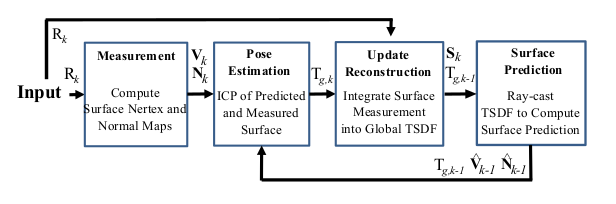
\includegraphics[width=12cm]{images/ch1/Newcombe11KinectFusion1}
\caption{Kinect Fusion Algorithm Pipeline \cite{Newcombe11Kinectfusion}}
\label{KFusionPipeline}
\end{figure}

Kinect Fusion has four main steps as illustrated in figure \ref{KFusionPipeline}. The first step named measurement, performs pre-processing on the depth data as well as generation of additional information for use by Kinect Fusion. Each depth map frame is first passed through a bilateral filter. From this, a dense vertex map (map of 3D points projected using a known projection matrix associated with the Kinect) is generated, as well as a normal map. For both the vertex and normal maps, a 3 level image pyramid is constructed. This makes the coarse to fine grain ICP technique possible. \\

Next, dense coarse to fine grain ICP is used to compute pose between the fused frames and the current frame. The authors exploit the fact that the transformation between frames is small because camera motion is slow when computing against every frame. With coarse-to-fine grain ICP they use the point-plane metric for pose optimization \cite{Rusinkiewicz02Real}. The ICP based pose estimation computes pose given both a predicted and measured depth map. \\

After estimating camera pose relating to the globally fused model, each frame must be integrated into that model. The Kinect Fusion algorithm uses a truncated signed distance function (TSDF) representation. This is a signed distance function volume where the distances for each voxel are capped by some value. The TSDF uses a volume resolution of $512\times 512\times 512$. They use the TSDF, rather than relying on a linear but accurate discrete SDF transform \cite{Rasch09Remarks} because of the computational complexity of calculating the discrete SDF of large scale volumes. \\

As mentioned, Kinect fusion uses pose prediction and fuses each depth map into the TSDF representation. In this way, they align and fuse each depth map to the global 3d reconstruction. In this way, a global loop closure method is not required. This may have a negative side effect by which some frames which have larger resolutions may be heavily quantized in order to fuse with the SDF, especially very thin surfaces/objects. These features may also be advantageous for ICP in estimating pose. 



\subsection{3D Reconstruction by Optimizing directly in the SDF}

In 2013, Bylow et al \cite{Bylow13Real} presented a novel method which reconstructs static indoor environments in real time using RGB-D data captured using the Asus Xtion Pro Live sensor. Their system is able to generate accurate 3D RGB coloured models of the environment in real-time by optimizing for 6 degrees of freedom in terms of accurate projection of new depth map frames into an existing global signed distance function model of the scene. Their method uses several Gauss Newton optimization with a signed distance function representation, these techniques are represented and processed using a laptop with an NVIDIA GPU. Unlike Kinect Fusion \cite{Newcombe11Kinectfusion}, this method optimizes directly in the signed distance representation, in which camera pose is computed by finding a rotation and translation (6-DoF) which minimizes the error of projecting depth images into the SDF. Compared with the ICP based method used by Kinect Fusion, this technique is shown to be more robust and accurate. It compares favourably to bundle adjustment but is much faster for small to mid sized scenes. Results are generated using the TUM RGB-D benchmark and SDF volume sizes $256^3$ and $512^3$ are used in evaluations. The authors note the algorithm may be able to handle large scale scenes if used in conjunction with other techniques \cite{Kaess11Isam2,Kummerle11G}. \\

This technique is efficient because the error to minimize can be checked using several look-ups since the SDF itself contains the distances from each voxel to the global model's actual surface. Because of this, the algorithm is classified as working within global space rather than frame-by-frame. Using the SDF to lookup depth map projection error, the camera pose is iteratively estimated and then the depth map is integrated into the SDF and colour information is stored in another volume. The pose estimation procedure begins by storing the first frame as a volumetric signed distance function. Then for each new depth frame, camera pose is computed, and based on this pose the frame is projected into the scene. Using a lie algebra based 6-DoF model \cite{Ma12Invitation} envisioned as a vector in $R^6$ representing camera pose, the error for a given pose may be computed as the squared error of the depth map transformed by the pose and projected into the signed distance function. Due to noise or missing data within the depth frame, this error may never be reduced completely, instead the best pose is iteratively computed using this model and the Gauss Newton non-linear optimization algorithm. \\

The SDF representation uses two volumes as in \cite{Curless96Volumetric}, one volume stores the average distances, the other stores the cumulative weights for each voxel. Bylow et al use these weights to handle occlusion and sensor uncertainty. When integrating a point into the SDF, tri-linear interpolation is used between eight neighbours to handle point coordinated made up of floating point numbers. During integration, each voxel is projected onto the image plane rather than ray case from the center of projection as in \cite{Newcombe11Kinectfusion}. This ensures that each voxel is visited once when updating the SDF, whereas in the ray casting approach, this may not necessarily be the case. \\

In computing the SDF for a given depth map, the exhaustive marching cubes algorithm is too slow, even the fast marching algorithm \cite{Baerentzen01Implementation} is not suited for real time discrete SDF generation. Instead, the SDF is approximated with either the point to point distance or point to plane distance functions. For final visualization, marching cubes is used \cite{Lorensen87Marching} on the final SDF. Colour is computed from the colour volume using a technique found used by Whelan et al \cite{Whelan13Robust}. Since the method by Bylow et al is based on optimizing the projection error using the SDF and only uses locations in its pose estimation procedure, it is independent to illumination. Given this, it will also fail in cases where only co-planar surfaces are visible, they mention that using colour information during tracking \cite{Kerl13Robust} may mitigate these concerns.


but kinect fusion generates synthetic depth images which are aligned to the current depth image using icp


\subsection{Sturm}

approach to SLAM for RGB-D cameras (eg. kinect)
computes dense 3d environment + computes camera pose
evaluated at different illuminations + camera speed conditions
evaluates 3 different features SIFT, ORB and SURF
system can deal with difficult data in common indoor scenarios and is fast enough for online operation
1st : extract features from color image data, match with previous frames
this gives point-wise 3d matches
then - RANSAC may be used to compute the transform between 3d frames
because frame-by-frame is not globally consistent
optimize the pose graph in a fourth step using the g2o solver [11] optimizes non-linear error functions
uses octomap [33] to generate a volumetric representation of the environment
uses datasets [29]
handles up to 50 deg per sec / ,43 meters per sec
voxelizes using octomap, uses 3d occupancy grid for output

SLAM used in robotics [30,22,10,6,15,9,23]
modern systems use ICP [2, 26, 27]
vslam [5, 16, 28, 14, 21] => get sparse keypoints,  
these simplify data association
sift[20, surf[1], orb[25]], sift gpu[32]


in monocular setting, the scale of the map cannot be  determined

stereo slam [17, 24] -> does not suffer from this
only accurate for textured surfaces, non-textured surfaces cannot be estimated with depth

Fioraio [7] presented a system which uses bunfle adjustment to align rgb-d data

henry [12] is similar to this work

uses sparse keypoint matches between color images as initialization to icp

icp often not necessary and expensive
icp only used if no keypoint matches found...

henry used sparse bundle adjustment [19], here 3d pose graph using [18] framework is used

henry put resulting into surfel representation, here volumetric voxel representation is used [33], can be used for robot localization, path planning and navigation [13]

figure 2 has a picture

front-end: keypoint det, match, sensor pose from ransac
back-end: optimizes poses with non-linear error function
	computes optimal sensor positions using a graph-based routine -> then the occupancy voxel grid map is computed
	
front-end details: 
uses opencv [3] for detection, description and matching of features SURF, SIFT and ORB [25], for SIFT: GPUSIFT[32]

ORB is based on FAST [25] and BRIEF[4]

ORB computes orientation from FAST corners and uses for descriptor extraction -> so it is more robust to viewpoint changes (faster than both sift and surf)

sets the hessian threshold to keep number of keypoints constant, too few keypoints and there may be not enough matches, too many and there may be too many false positives

then the transformation of camera pose can be computed from these correspondences [31]


because of synchronization at the shutters of infrared and color camera and due to interpolation at depth jumps
plus because features often lie at object borders, 3d features positions are prone to be at a wrong depth making robust estimation of transformations highly non-trivial

RANSAC known to cope with noise data [8]
points considered inliers if after transformation their distance is < 3cm

then, the inliers are used to compute a finer representation, these steps are repeated where most inliers are kept

















[BG Bylow]

bundle adjustment using features over many views with [13 \cite{Klein07Parallel} , 2 \cite{Agarwal09Building}] with sparse 3d models generated

algorithms to compute dense depth maps from image data [10 \cite{Hirschmuller05Accurate} , 21 \cite{Stuhmer10Real}]

newcombe [18 \cite{Newcombe11Kinectfusion} ] -> impressive results using sdfs to represent reconstruction, and icp for camera tracking

whelan [24 \cite{Whelan13Robust}] estended with rolling reconstruction volume and color fusion, evaluated alternative methods for visual odometry estimation

pure visual odometry induces significant drift, so matching with global model is their preference

novel method of estimating camera motion directly based on the SDF, key insight : sdf encodes distance to surface

do not need downsampling in case of icp to achieve real time performance

comparable to the feature based rgb-d slam [8 \cite{Endres12Evaluation}]

icp[4 \cite{Besl92Method}]

graph slam use motion estimates as input to construct and optimiza a pose graph[15 \cite{Kummerle11G}] these methods render a joint map only after pose graph optimization

this map is generally not used for further optimization

the resulting maps are often represented as occupancy grid maps or octrees [25 \cite{Wurm10Octomap}]

henry [9 \cite{Henry10Rgb}], applied graph slam to rgb-d data, using visual features + icp combo [8] also did a similar system, on benchmark [22 \cite{Sturm12Benchmark}]

[18 \cite{Newcombe11Kinectfusion} dense 3d recon possible with realtime, 

sdf[7 \cite{Curless96Volumetric}]

KF: for each image:
it renders a point cloud from the sdf at the previous pose using ray tracing and aligns this with the depth image


point correspondences are found using projective data association [5 \cite{Blais95Registering}] and the point to plane distance

Kin-Fu open source implementation available in the PCL library

(icp only minimizes error on point clouds, some other approaches minimize photometric error [20 \cite{Steinbrucker11Real}, 12 \cite{Kerl13Robust}]

or combinations of both [23 \cite{Tykkala11Direct}]) -> these did not perform 3d reconstruction

whelan integrated these methods with kinect fusion [24 \cite{Whelan13Robust}]

Canelhas [6 \cite{Canelhas12Scene}] did masters thesis an approach for camera tracking, similar to this
his focus concentrates on object detection and recognition in an sdf and no thorough evaluation was performed

Kubacki [14 \cite{Kubacki12Registration}] showed how an sdf can be used to estimate camera pose, only on synthetic data without a comparative evaluation

[19 \cite{Ren12Unified}] demonstrated sdf based object tracking, based on known models

presented by Bylow: direct approach to camera tracking on sdfs


stable enough for use with quadcopter























[Background from KF]

area promises new augmented reality and mixed reality applications

SFM and MVS (multi view stereo) has given good results : camera tracking  and sparse reconstructions [10] \cite{Fitzgibbon98Automatic}, \cite{Seitz06Comparison} [24] 

SLAM has focused on real time markerless tracking and live scene reconstruction based on a single sensor RGB eg. MonoSLAM[8] \cite{Davison03Real} which is less accurate than PTAM [17] \cite{Klein07Parallel}  but these only produce sparse reconstructions

some methods have grown to combine PTAM's camera tracking ability with MVS-style reconstructions [19/26] (\cite{Newcombe10Live}/\cite{Stuhmer10Real})

recently: iterative image alignment has been used to replace features in tracking [20] \cite{Newcombe11Dtam}

this scene is promising: but monocular based dense 3D reconstruction is difficult and requires suitable camera motion and scene illumination

camera technologies have also been evolving: enter the world of new depth cameras or rgb-d cameras,
these have become available to consumers and may soon be found in mobile technologies \cite{Zhang12Microsoft}

first real-time rgb-d depth sensor : with this system users can wave around the device to generate smooth, continuously updating, fully reconstructed data: using only depth, 6dof are tracked

works in full darkness : mitigating issues for passive cameras: [17 \cite{Klein07Parallel} /19 \cite{Newcombe10Live} /26 \cite{Stuhmer10Real}] and other rgb systems [14 \cite{Henry10Rgb}]

[XYZ]

kw : dense volumetric reconstruction

GPGPU kw: is one of their design keys, their system can perform in real time at above these frame rates

they perform qualitative analysis

Kinect: incorporates a structured light based depth sensor, uses an on board ASIC generating an 11-bit 640x480 depth map at 30hz

depth images often contain holes : this is an issue (caused by no structured light could be read on the surface, certain materials, which do not reflect infra-red light (very thin structures or surfaces at incendence angles

when moving fast, the device can also experience motion blur, this leads to missing data

then they do  reviews on:
	slam, dense tracking, surface representations, previous work with joint tracking and modelling using depth sensors

[Background]

early sfm algorithms: either accumulated drift (computing motion) [2 \cite{Beardsley97Sequential} ] or performed loop-closure using off-line optimization 

The first monocular slam system [8 \cite{Davison03Real} ] was capable of producing globally consistent maps in real time with hand-held camera used probabilistic filtering of camera and scene feature estimates

limited to in-door office environments because it requires large state vectors which grow with scene size
sparse feature maps lead to poor accuracy

then systems which split tracking and mapping (global optimization) -> approach by PTAM system [17 \cite{Klein07Parallel}]
: real time mono slam in work spaces -> basically it is just bundle adjustment (which is the least squares solution to camera and feature optimization (theirs chooses features dynamically over the frame range)

their tracking system runs in parallel at frame-rate speeds, and performs robust n-point pose estimation with feature matching

compared to filters much more features can be packed into the map[25 \cite{Strasdat10Real} ]

PTAM = realtime results as accurate as off-line ones

PTAM produces sparse maps - not like our project

some algorithms can use PTAM tracking in conjunction with dense reconstruction computing module based on multi-view stereo

[19 \cite{Newcombe10Live}] uses dense optical flow with PTAM like tracking for dense recon

this relies on camera poses coming from PTAM

[26 \cite{Stuhmer10Real}] do the same with near real time depth map calculation

DENSE TRACKING AND MAPPING by Scan Alignment

dense sensor based 3d reconstruction research has continued using lasers and depth sensors

typically : minimize distance measures between all data rather than feature extraction and matching

6dof camera alignment and 3d surface reconstruction techniques developed in the graphics domain, here ICP is the most important
ICP @ [3 \cite{Besl92Method} ]

ICP is a non-linear optimization problem where approximations are found using the closest points currently for each
set

distance metrics have been researched using the point-plane metric [5 \cite{Chen92Object}]

[\cite{Chen92Object} 5] improves convergence rates, used for surface reconstructions which have normal data

computing closest points using ICP is expensive, there is projective data association algorithm [4 \cite{Blais95Registering}]

can be used for data in projective form (2d image where each image is a 3d point)

can reduce icp set to possible set of points or with a coarse to fine scheme

SLAM may use ICP to estimate camera changes

Dense 3D scene representations:

occupancy mapping : use a grid to store data

[9 \cite{Elfes87Sensor}] uses a Bayesian probability of occupancy to measure whether should be added to the grid

also can used signed distance functions [9 \cite{Elfes87Sensor}] (SDF), it can be used to fuse partial depth scans, whilst mitigating
issues relating mesh-based reconstruction algorithms

SDF represents : surface interfaces as 0, positive values that increase with distance from the nearest surface
and occupied space using a negative value

more robust to noise version of SDF -> [30 \cite{Zach07Globally} ]

SDF can be visualized by first converting to mesh and rendering ( use marching cubes [18 \cite{Cubes87High}]) or it can be directly ray cast [21 \cite{Parker98Interactive}]

[23 \cite{Rusinkiewicz02Real}] used frame-by-frame ICP with occupancy grid, users can scan in small objects by rotating the objects with their hand
works @ 10hz, issue: does not do global optimization, cannot do large scenes . final models are optimized using [7 \cite{Curless96Volumetric}]
sdf fusion in real time may be possible

sdf can be used for globally satisfying reconstruction

small scale reconstructions:
	[28 \cite{Weise09Hand}] -> produces high quality scans using a fixed ToF sensor
	[6 \cite{Cui103d} ] demonstrate a moving handheld ToF scanner

Octomap [29 \cite{Wurm10Octomap}] -> 3d reconstruction using occupancy grid style 

[14 \cite{Henry10Rgb}] uses rgb-d with kinect by frame by frame icp : feature matching is used with graph optimization for loop closure and global consistency -> global fusion presents better performance








































\ref{Newcombe11Kinectfusion}

\subsection{RGB-D Sensor Feature Based Systems}
RGB-D SLAM systems use both depth and image data and are capable of generating dense 3D reconstructions. Many of these methods rely on feature matching techniques \cite{Engelhard11Real,Henry10Rgb,Endres12Evaluation}. RANSAC is often used to filter outliers for the estimation of camera parameters\cite{Engelhard11Real,Henry10Rgb,Endres12Evaluation}. Another method which has also been used extensively in the area is Iterative Closest Point (ICP) \cite{Engelhard11Real,Henry10Rgb,Bylow13Real,Newcombe11Kinectfusion,Stuckler12Robust,Izadi11Kinectfusion}. ICP iteratively registers point cloud data, and is used to refine camera parameter estimates. A method named KinectFusion was proposed by Newcombe et al \cite{Newcombe11Kinectfusion} which uses RANSAC and a GPU implementation of IPC. Whelan et al \cite{Whelan12Kintinuous} extended this method allowing it to map larger areas using Fast Odometry From Vision (FOVIS) over ICP. Bylow et al \cite{Bylow13Real} improved the ICP approach by registering data using a signed distance function.
\subsection{Non-Feature Based Methods}
Several RGB-D SLAM systems are also non-feature based \cite{Weikersdorfer14Event,Izadi11Kinectfusion,Kerl13Dense}. Weikersdorfer et al \cite{Weikersdorfer14Event} presented a novel sensor system named D-eDVS along with an event based SLAM algorithm. The D-eDVS sensor combines depth and event driven contrast detection. Rather than using features, it uses all detected data for registration. Kerl et al \cite{Kerl13Dense} proposed a dense RGB-D SLAM system which uses a probabilistic camera parameter estimation procedure. It uses the entire image rather than features to perform SLAM.
\subsection{Summary}
As is evident from the current literature, SLAM typically relies on feature matching and RANSAC. However, these approaches fail when there are too few features, when feature confusion occurs or, when features are non-stationary due to object motion. As the extent of random feature displacement becomes more global the effectiveness of these approaches diminishes. Feature matching also dominates in image registration. However, Fourier based methods have been shown to work well under larger rotations and scales \cite{Gonzalez11Improving} whilst being closed form, insensitive to object motion and scaling naturally to GPU implementations. Accordingly, we propose a novel, closed form Fourier based SLAM method.

Simultaneous localization and mapping (SLAM) has applications in many fields including: robotics, business, architecture and engineering, and science. Its goal is to generate a map (2D birds-eye view, or 3D) of an environment captured by camera and/or other means. In this work we focus on monocular systems, or systems which generate location and mapping data using information generated by a single basic video camera. To this end, current methods rely on the computation of the fundamental and essential matrices. These feature matching techniques fail in cases where features are not stable or where feature confusion occurs. 

It has been shown [1] that using volume registration to compute dense 3D maps is not only independent of feature matching, but it is a closed form solution and is robust to noise and object motion. However, this method requires RGB-D video input provided by special hardware. In this paper we present preliminary results in applying volume registration to generate dense 3D maps from monocular video data. To achieve this, disparity maps are generated between video frames. This data is then used as input for the RGB-D volume registration method.

\section{Feature Matching and RANSAC}

\section{Iterative Closest Point}

\section{Fourier Based Registration}

\section{3D Data Compression Schemes}

\subsection{Model Compression}

The Feature-Oriented Geometric Progressive Lossless Mesh coder (FOLProM) \cite{Peng10Feature} is a state of the art codec which is progressive. It also aims to be an effective low-bitrate codec. It classifies segments of the mesh as being visually salient or not. Salient segments are preserved more during compression compared to non-salient ones. \\

\subsection{Spectral Compression}

Karni and Gotsman \cite{Karni00Spectral} proposed a lossy method which compresses a spectral representation of a mesh. This algorithm generally partitions the mesh and compresses each partition separately since it does not work on large meshes. Encoding a basis function for each partition, coefficients are quantized, truncated and entropy coded. Results show this method outperforms the valence method \cite{touma98triangle} at coarse quantization levels. Bayazit et al. \cite{Bayazit103DMesh} also developed a progressive method based on spectral compression. This method is based on the region adaptive transform in the spectral domain and is advertised as a current state of the art lossy 3D data compression method. \\

\subsection{Wavelet Methods}

A lossy wavelet based compression system was proposed by Khodakovsky et al \cite{Khodakovsky00Progressive}. This technique samples the mesh, and uses the wavelet transform to decorrelate the data. Coefficients are quantized and stored in a structure called a zero tree which increases compression performance. This method is shown to outperform the valence method. Other wavelet approaches \cite{Guskov00Normal,Khodakovsky04Normalmesh} also sample the mesh and use a multi-resolution representation in which the data is described using local normal directions on the mesh surface.

Gu et al \cite{Gu02Geometry} devised a solution for representing 3D models as 2D images which are then compressed using state of the art image compression methods (based on wavelets). To form this representation, the mesh is cut along a network of edge paths, opening the mesh into a topological disk, which is then sampled onto a 2D grid. Each pixel in the image has a corresponding coordinate in the model, with pixel neighbourhoods describing connectivity. Comparisons with the method by Khodakovsky et al reveal the geometry image codec does not have as high compression performance.



\section{Conclusion}

 % The Literature Review
%\begin{savequote}[8cm]
  ``I have not failed. I've just found 10,000 ways that won't work.''
  \qauthor{Thomas Edison}
\end{savequote}
\makeatletter
\chapter{Methodology}

\section{Introduction}

intro about this section...

\section{Fourier Volume Registration}

\subsection{Recovery of Translation Values}

Given a volume $V_1$ and a spatially shifted version of it $V_2$, the offset along each axis, $(x,y,z)$ may be recovered if a suitable correlation between the two volumes can be found. \\

The measure of correlation between $V_1$ and $V_2$ can be found by shifting $V_1$ and $V_2$'s mean values to zero, then summing the element-wise multiplication of $V_1$ by $V_2$. Equation \ref{eqn:CorrelationEquation} computes this correlation measure.

\begin{equation} \label{eqn:CorrelationEquation}
\sum_{z=0}^{N}\sum_{y=0}^{N}\sum_{x=0}^{N}(V_1(x,y,z)-avg(V_1)) \times (V_2(x,y,z)-avg(V_2))
\end{equation}

Using this measurement, two volumes which are similar in signal shape (element-wise-value to location correspondence) will give a larger measure of correlation than two volumes with a differing signal shape. If the volumes are first normalized we can regard volume $x$ is more aligned with volume $y$ than with volume $z$ given $x$ correlated with $y$ gives a larger value than $x$ correlated with $z$. \\

Cross-correlation searches over a space of translation parameters and outputs the optimal translation to align two volumes. It is optimal in the sense of correlation measurement. This is used as a best guess in terms of the alignment of the two volumes. It can be thought of as the optimization of parameters $x,y,z$ in equation \ref{eqn:CrossCorrelationEquation}.

\begin{equation} \label{eqn:CrossCorrelationEquation}
CrossCorrelate(Transform(V_1, x,y,z), V_2)
\end{equation}

Since we typically do not know the range of translation values $x,y,z$ to optimize for, we take into account the range from $[0,N]$ where $N$ is the width/height/depth of the volume. This gives a complexity of $N^6$. This is too computationally complex for practical volume sizes. Therefore, we use the properties of the Fourier Transform to reduce computational complexity.


 

Using the properties of the Frequency domain, we can efficiently recover the optimal alignment translation parameters using a function called $PhaseCorrelation$ (Eq. \ref{eqn:PC_basic}). This function takes two volumes as input and returns the best alignment translation between them in terms of maximizing correlation.
\begin{equation} \label{eqn:PC_basic}
(x, y, z) = PhaseCorrelation(V_x, V_y)
\end{equation}
The $PhaseCorrelation$ function first applies 3D FFTs to volumes, $V_1$ and $V_2$, converting them into the frequency domain, i.e. $F_{1_{x,y,z}} = FFT(V_1)$ and $F_{2_{x,y,z}} = FFT(V_2)$. Taking the normalised cross power spectrum using Eq. \ref{eqn:PHCOR_eq} based on these frequency domain volumes computes the frequency domain of a new volume called the phase correlation volume. \\


\begin{equation} \label{eqn:PHCOR_eq}
F_{3_{x,y,z}} = \frac{F_{1_{x,y,z}} \circ F_{2_{x,y,z}}^*}{ | F_{1_{x,y,z}} \circ F_{2_{x,y,z}}^* | }
\end{equation}

Here, $\circ$ is an element-wise multiplication and $|x|$ is the magnitude function. Taking the inverse FFT of the frequency domain of the phase correlation volume, $F_3$ gives the phase correlation volume itself, $V_3$ ($V_3 = FFT^{-1}(F_3)$). The location of the peak value in the phase correlation volume $V_3$, $(x_1, y_1, z_1)$ gives the shift between the $V_1$ and $V_2$. The phase correlation volume is typically noisy making the peak difficult to locate. Each in the phase correlation volume evaluates the correlation between $V_1$ (translated by the location of the peak) and $V_2$.


\subsection{Recovery of Y-Axis Rotation}

\subsection{Recovery of Scale}

\subsection{Full Recovery of 3D Rotation}




\section{Fourier Volume Registration based 3D Reconstruction}


In this section we describe the general technique of recovering pose estimation via Fourier volume registration techniques. Several methods may be used and each has its own advantages and disadvantages and suitability depends on pose restriction, camera accuracy, noise levels and input data. 


\subsection{A Volume Registration based 3D Reconstruction Pipeline}

\label{METHOD_SECLL}
The proposed 3D reconstruction method consists of various steps. First each frame $f_i$ that is captured, consisting of a colour and depth image pair is projected into 3D space, forming colour point cloud $points_i$ and re-sampled into a volume $V_i$. Then, the transform parameters between pairs of volumes $V_i$ and $V_{i+1}$ are estimated using $VolumeRegister_{\theta \varphi t_x t_y t_z}$ shortened to $VR_{\theta \varphi t_x t_y t_z}$. These parameters are used to update transformation matrix $M$. The points corresponding to $f_2$ ($points_1$) are then transformed using the updated $M$ matrix and added to the cumulative $PointCloud$ database. Two lists, $Cameras$ and $Poses$, are also updated to track camera pose and location per frame. This basic procedure is given in listings \ref{algorithm:PCSLAM} and elaborated upon in subsequent subsections.
\begin{figure}
\begin{lstlisting}[language=c++,caption=Phase Correlation Based SLAM Algorithm,label=algorithm:PCSLAM,mathescape,basicstyle=\ttfamily]
$f_1$ = ReadFrame();
$PointCloud$ = project($f_1$);
$M$ = IdentityMatrix();
$Camera$ = $[0, 0, 0]^T$;
$Pose$ = $[0, 0, 1]^T$;
$Cameras$ = $\left[Camera\right]$, $Poses$ = $\left[Pose\right]$;
while(more frames){
	$f_2$ = ReadFrame();
	$points_1$ = project($f_2$);
	$points_2$ = project($f_1$);
	$V_1$ = ResampleVolume($points_1$);
	$V_2$ = ResampleVolume($points_2$);
	$(\theta, \varphi, t_x, t_y, t_z) = VR_{\theta \varphi t_x t_y t_z}(V_1, V_2)$;
	$M = M \times$TransformMat($(\theta, \varphi, t_x, t_y, t_z)$);
	$points_1$ = Transform($points_1$, $M$);
	$PointCloud$ = $PointCloud \cup points_1$;
	$Camera$ = $M^{-1} \times Camera$;
	$Pose$ = $M^{-1} \times Pose$;
	$Cameras.add(Camera)$;
	$Poses.add\left(\frac{Pose-Camera}{|Pose-Camera|}\right)$;
	$f_1$ = $f_2$;
}
\end{lstlisting}
\end{figure}


The input to our method is a color and depth image pair, $f(u,v)$ and $g(u,v)$ obtained using an Asus Xtion PRO LIVE sensor at a resolution of $640 \times 480$. Each pixel is projected into 3D space using $X_{u,v} = \frac{(u - c_x)Z_{u,v}}{f}$, $Y_{u,v} = \frac{(v - c_y)Z_{u,v}}{f}$ and $Z_{u,v}$ = $g(u,v)$. 
Here, $[c_x c_y]^T$ represent the center of the image whilst $f$ represents the focal length, defined as $525.0$. The point clouds generated by projecting these images are then quantized into image volumes. Results reported in this paper were obtained using volumes of $384^3$ voxels in size.

\begin{figure*}[t]
\centering
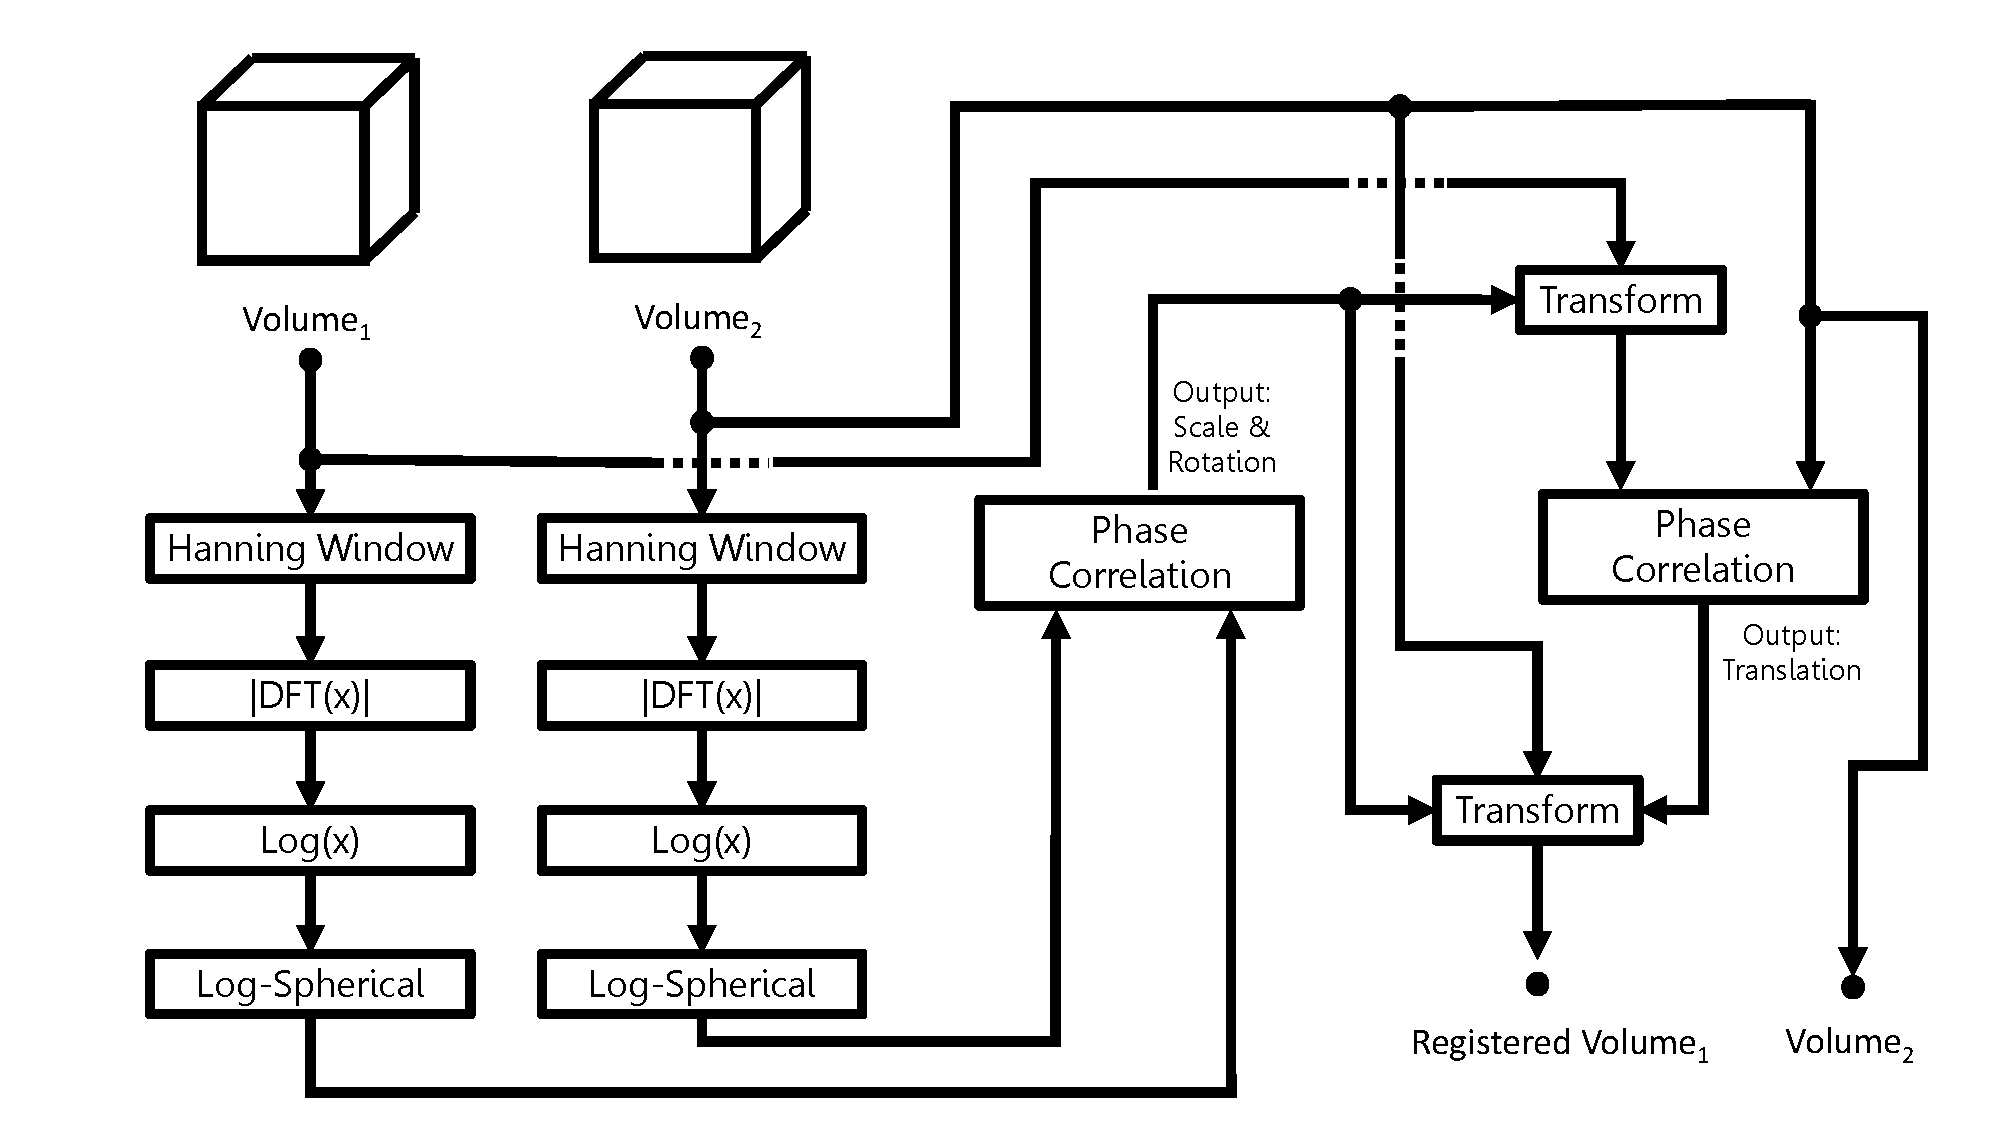
\includegraphics[width=6.0in]{images/ch2/pipeline2}
\caption{System Diagram for Registration Process}
\label{fig:PIPELINE}
\end{figure*}


\subsection{Error metrics}

In order to evaluate the accuracy of volume registration we use several error metrics including: Hausdorff error, mean squared error and the percentage of matched voxels. We describe mathematically those techniques here. All measurements are based on a simple function which computes the nearest neighbour for a given 3D point or voxel given a volume (or collection of 3D points). We define such a function, named nearest-neighbour in equation \ref{eqn:NN}.

\begin{equation} \label{eqn:NN}
NN(p, V) =  \{ q \in V | (Dist(q, p) < Dist(k, p))  \forall k \in V \}
\end{equation}

This function retrieves the closest corresponding point given a query point $p$ and a volume or point cloud of points, $V$. This function can be used to provide omni-directional error functions based on Hausdorff, mean squared and percentage accuracy error metrics.

Here some one-way error functions are described. The one was Hausdorff error is defined in \ref{eqn:HDOW} 

\begin{equation} \label{eqn:HDOW}
\sum_{k=0}^{N} Dist(P_k, NN(P_k, Q))
\end{equation}

\subsection{Reconstruction Integration}

Using the techniques of registration described in the above sections, there are several techniques which may be used to integrate these registered data. In most experiments we use the volume integration to combine the registered data in a single global model. We also propose several techniques for data representation and evaluate their abilities (see section \ref{sec:3DDataRepresentations}). As for the typical volume integration used, we create volumes with dimensions of $512\times 512\times 512$, although larger sizes may be used for increased accuracy. Once a frame is registered, it is projected into the volume. \\

This projection follows the following formula


\begin{equation} \label{eqn:volIntegration}
\begin{split}
x^{1} & = floor((x - frameCenter_x) \times scalar + volumeCenter_x) \\
y^{1} & = floor((y - frameCenter_y) \times scalar + volumeCenter_y) \\
z^{1} & = floor((z - frameCenter_z) \times scalar + volumeCenter_z)
\end{split}
\end{equation}

$frameCenter$ is the center of the projected frame space and $volumeCenter$ is the center of the integration volume, typically scalar is set to 1 or is used to trade-off resolution and map size. An example of an integration process is illustrated in figure XFDF. 


\subsection{Advantages and Disadvantages}





\subsection{Fourier Volume Registration}

\subsubsection{Volume Representation}

\subsubsection{Phase Correlation and Recovery of Translation Values}

\subsubsection{5-DoF Registration using FFT}

Figure \ref{fig:PIPELINE} shows a functional block diagram of our method. The input data are two 3D volumes ($Volume_1$ and $Volume_2$) and the output is the transformation matrix required to register the two volumes. The volumes are first Hanning windowed. Next, a translation independent representation is obtained for each by taking the magnitude of their 3D FFTs. Then a log function is applied to the resulting magnitude values, improving scale and rotation estimation \cite{Gonzalez11Improving}. Following a log-spherical transformation, 3D phase correlation is performed to find the global rotation and scale relationship between $Volume_1$ and $Volume_2$. $Volume_1$ is then inversely transformed by the rotation and scale parameters, leaving only the translation to be resolved. This is found by applying phase correlation again between the transformed $Volume_1$ and $Volume_2$. 
\subsection{Phase Correlation}
Given a volume $V_1$ and a spatially shifted version of it $V_2$, the offset can be recovered using $PhaseCorrelation$ (Eq. \ref{eqn:PC_basic}). This function takes two volumes as input and returns the translation between them.
\begin{equation} \label{eqn:PC_basic}
(x, y, z) = PhaseCorrelation(V_m, V_n)
\end{equation}
The $PhaseCorrelation$ function first applies 3D FFTs to volumes, $V_1$ and $V_2$, converting them into the frequency domain, i.e. $F_{1_{x,y,z}} = FFT(V_1)$ and $F_{2_{x,y,z}} = FFT(V_2)$. Taking the normalised cross power spectrum using Eq. \ref{eqn:PHCOR_eq} completes the Phase correlation function. 
\begin{equation} \label{eqn:PHCOR_eq}
F_{3_{x,y,z}} = \frac{F_{1_{x,y,z}} \circ F_{2_{x,y,z}}^*}{ | F_{1_{x,y,z}} \circ F_{2_{x,y,z}}^* | }
\end{equation}
Here, $\circ$ is an element-wise multiplication and $|x|$ is the magnitude function. Taking the inverse FFT of $F_3$, gives the phase correlation volume $V_3$ ($V_3 = FFT^{-1}(F_3)$). The location of the peak value in $V_3$, $(x_1, y_1, z_1)$ gives the shift between the $V_1$ and $V_2$. The phase correlation volume is typically noisy making the peak difficult to locate. 
\subsection{Recovering Scale, Rotation and Translation Parameters}
If $V_1$ and $V_2$ are instead rotated and scaled versions of the same volume, such that they are related by some translation $(t_x, t_y, t_z)$, y-axis rotation $\theta$, and scale $\varphi$. Further action is required to recover translation parameters. The first step, given two volumes $V_1$ and $V_2$ of size $N^3$ is to apply a Hanning windowing function (Eq. \ref{eqn:Hann}). 
\begin{equation} \label{eqn:Hann}
\scriptstyle
HW_{x,y,z} = \frac{1}{2}\left(
1 - cos \left(
\frac{2\pi
\left(
\sqrt{\left(\frac{N}{2}\right)^3} -
\sqrt{
\left(x-\frac{N}{2}\right)^2 + \left(y-\frac{N}{2}\right)^2 + \left(z-\frac{N}{2}\right)^2
}
\right)
}
{2\sqrt{\left(\frac{N}{2}\right)^3} - 1}
\right)
\right)
\end{equation}
The rotation and scale factors are recovered first using a translation independent representation of the volumes using the Fourier shift theory. For this, the magnitude of the FFT of the volumes is taken, $M_1 = |FFT(V_1)|$, $M_2 = |FFT(V_2)|$. The zero-frequency of both $M_1$ and $M_2$ is shifted to the center of the volume and the log of the result is taken $M'_1 = Log(M_1)$, $M'_2 = Log(M_2)$ which reduces noise on the phase correlation volume. A log-spherical transform is then used to turn rotation and scaling into translation for both $M'_1$ and $M'_2$. Eq. \ref{eqn:Log_Spherical} shows the corresponding log-spherical space coordinate $(X_{log-spherical}, Y_{log-spherical}, Z_{log-spherical})$ for a given $(x,y,z)$ euclidean space coordinate.
\begin{equation} \label{eqn:Log_Spherical}
\begin{split}
X_{log-spherical} & = \frac{atan\left(
\left(\frac{x-\frac{N}{2}}{\sqrt{x^2+y^2+z^2}}\right)
\left(\frac{y-\frac{N}{2}}{\sqrt{x^2+y^2+z^2}}\right)^{-1}
\right)N}{360}\\
Y_{log-spherical} & = \frac{acos\left(
\frac{y}{\sqrt{x^2+y^2+z^2}}
\right)N}
{180} \\
Z_{log-spherical} & =\frac{log\left(\sqrt{x^2+y^2+z^2}\right)N}{log\left( \frac{N}{2.56} \right)} \\
\end{split}
\end{equation}
The log-spherical transforms of $M'_1$ and $M'_2$ are then phase correlated to find the shift between them, $(x_{M'},y_{M'},z_{M'}) = PhaseCorrelation(M'_1, M'_2)$. The rotation $\theta$ and scale $\varphi$ factors between $V_1$ and $V_2$ can then be found from the shift parameters using Eq. \ref{eqn:ROTATIONSCALEFROMXM} . 
\begin{equation} \label{eqn:ROTATIONSCALEFROMXM}
\begin{split}
\theta & = \frac{-360x_{M'}}{N}\\
\varphi & = e^{
-\left(
2.56^{-1}N
\right)z_{M'}N^{-1}
}
\end{split}
\end{equation}
Using $\theta$ and $\varphi$, $V_1$ can now be inverse transformed (using $(\frac{N}{2}, \frac{N}{2}, \frac{N}{2})$ as the origin). This aligns $V_1$ and $V_2$ with respect to scale and y-axis rotation. The translation parameters $(t_x, t_y, t_z)$ can then be found using phase correlation as given in Eq. \ref{eqn:FINALTRANS}.
\begin{equation} \label{eqn:FINALTRANS}
(t_x, t_y, t_z) = PhaseCorrelation(scale(rotate(V_1,\theta),\varphi), V_2)
\end{equation}
The complete function to recover translation, rotation and scaling, combining equations \ref{eqn:PHCOR_eq}-\ref{eqn:FINALTRANS} as is denoted in \ref{algorithm:PCSLAM} is \ref{eqn:FULLPC}.
\begin{equation} \label{eqn:FULLPC}
(\theta, \varphi, t_x, t_y, t_z) = PhaseCorrelation_{\theta \varphi t_x t_y t_z}(V_m, V_n)
\end{equation}


\subsubsection{Filtering Techniques in FFT based Volume Registration}

\subsection{Fast Fourier Volume Registration}

\subsubsection{Improving Speed : A 2D Case}

\subsubsection{Improving Speed : A 3D Case}

To reduce complexity we focus on areas which require the most computation time. In the earlier defined Fourier based reconstruction technique, this occurs in the two 3D phase correlations which need to be computed. We describe the method of reduction here; a block diagram for this technique is given in figure \ref{fig:PIPELINE3}. We refer to this method as fast volume registration (FVR) in reference general volume registration (VR). The speedup begins by computing the 3D DFT of both input volumes and taking the magnitude of these. Rather than directly performing a 3D log-spherical transform and a 3D phase correlation operation on these volumes, we use a novel transform we call a spherical-map transform (details in \ref{SMTransform}).\\

\begin{figure*}[t]
\centering
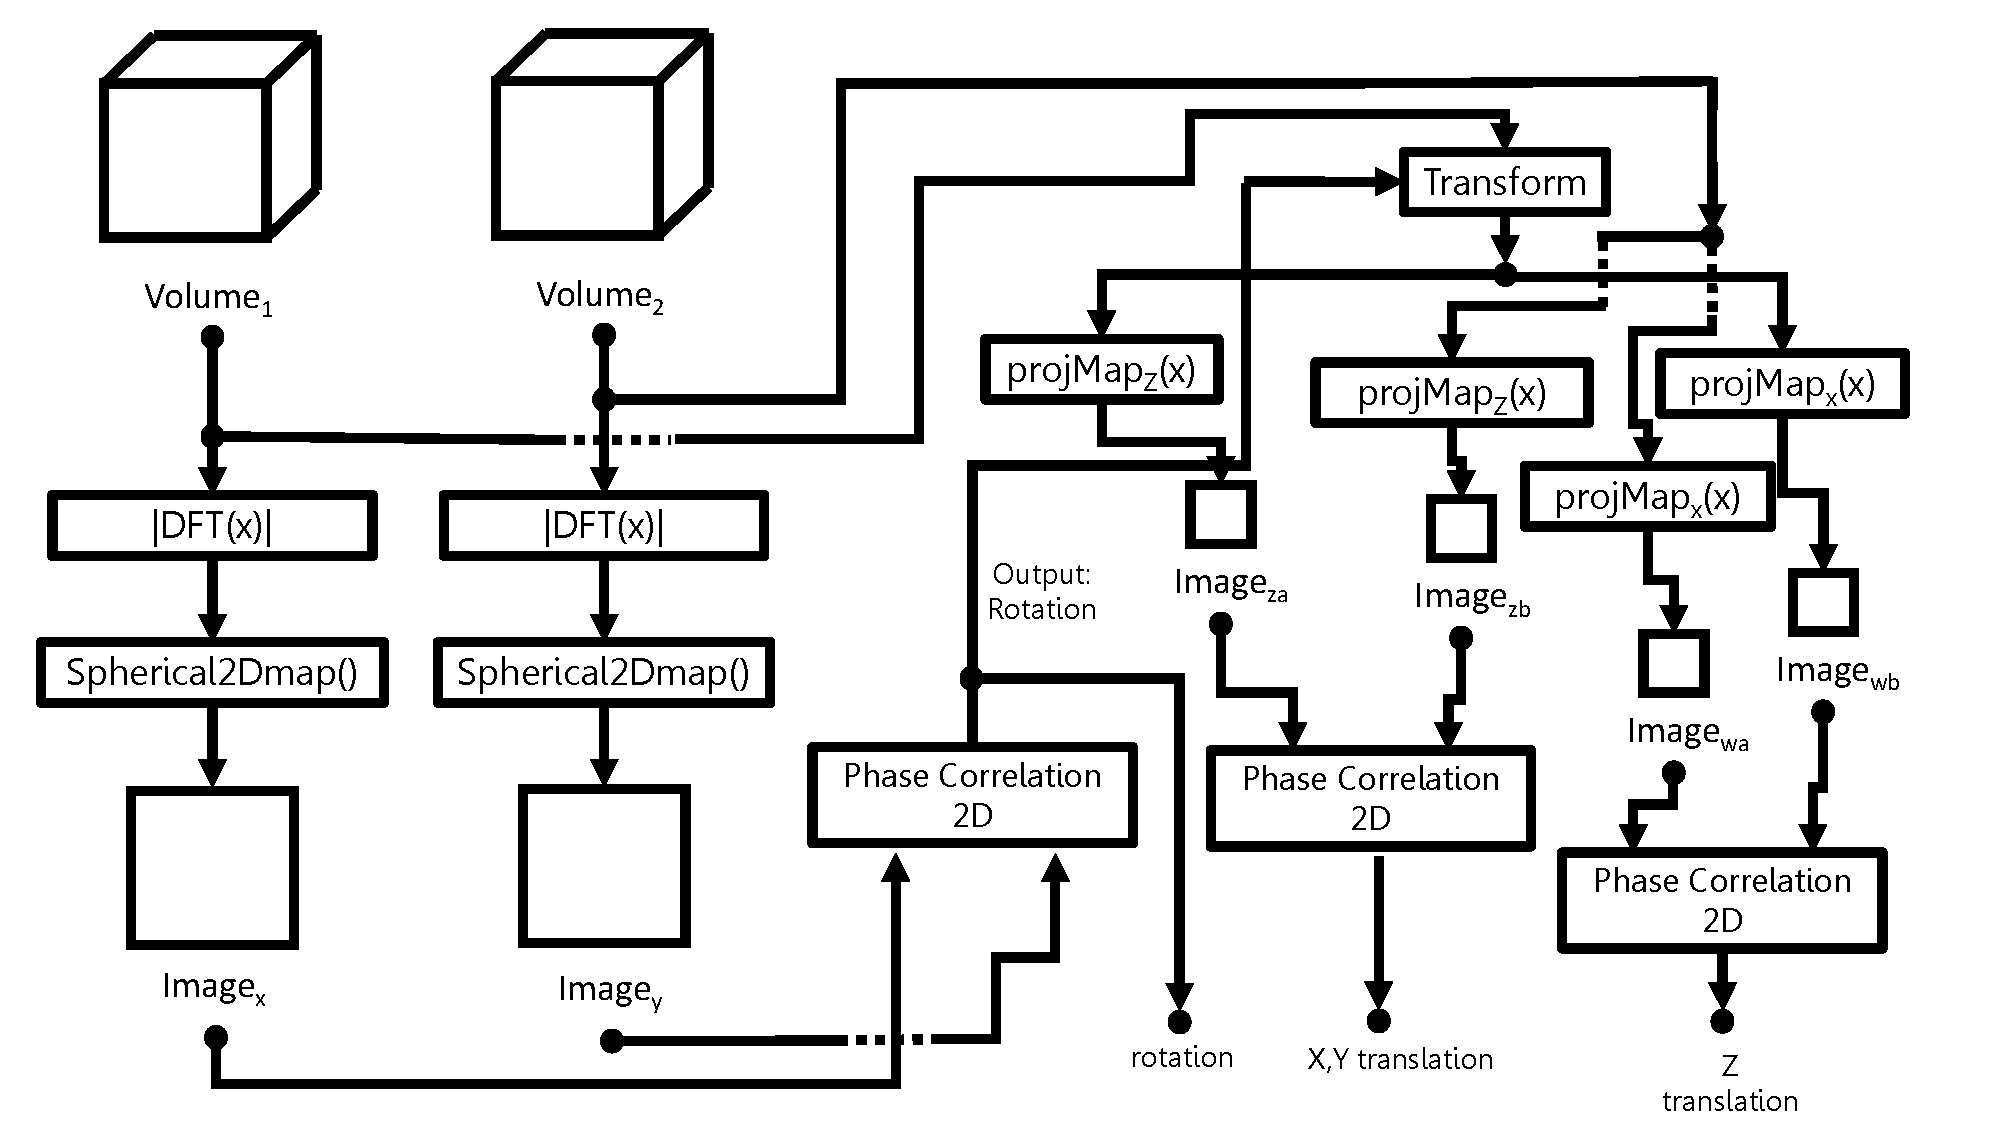
\includegraphics[width=6.0in]{images/ch2/pipeline3}
\caption{System Diagram for Fast Volume Registration}
\label{fig:PIPELINE3}
\end{figure*}

This transform converts rotation into translation whilst simultaneously unfolding the 3D space down to 2-dimensions. After this, a 2D phase correlation that requires significantly less processing compared with the 3D counterpart is used to compute the rotation. Next, having obtained the rotation parameter, the rotation is eliminated from the transformation by rotating the first volume by this parameter. The two volumes are then passed through two orthogonal projection mapping functions. This also converts the volumes to 2D space. We use two transforms for both volumes, one projection along the x-axis, another along the z-axis. Once the x-axis projections of both volumes are complete, we can do another 2D phase correlation to give us the z-translation. The 2D phase correlation of the z-axis projections gives us the x and y axis translations separating the original volumes. The final output of this method gives the rotation and translational shifts between the input volumes. The projections add little complexity to the overall algorithm and since 2D phase correlation operations are used in place of 3D ones, much computation time is reduced.

\subsection{Spherical-map transform}
\label{SMTransform}
The spherical map transform both reduces the 3D volume to a 2D image, and any rotation about the y-axis becomes x-axis translation in the output image. An example of the bunny model and the spherical-map transform of this model is given in figure \ref{fig:smtExample}, the mathematics are defined in equations \ref{eqn:invLPFuncs} and \ref{eqn:smtUpdate}. Given a coordinate in 2D Cartesian space x,y, we compute the ray $[Ray_x Ray_y Ray_z]^T$ from the volume center and sum up the voxel values along the ray (equation \ref{eqn:smtUpdate}). \\


\begin{equation} \label{eqn:invLPFuncs}
\begin{split}
Ray_x(x,y) & = cos\left(\frac{360x}{N}\right)sin\left(\frac{180y}{N}\right)  + \frac{N}{2} \\
Ray_y(y) & = cos\left(\frac{180y}{N}\right) + \frac{N}{2} \\
Ray_z(x,y) & = 	sin\left(\frac{360x}{N}\right)sin\left(\frac{180y}{N}\right) + \frac{N}{2}
\end{split}
\end{equation}

\begin{equation} \label{eqn:smtUpdate}
Im_{x,y} = \sum_{r=1}^{(2^{-1}N)^{1.5}}{Vol(Ray_x(x,y)r, Ray_y(y)r, Ray_z(x,y)r)} 
\end{equation}

This is process essentially sums up the values along a given ray defined by scaling spherical coordinates and adding up the values intersecting the ray. The resulting image, maps 3D y-axis rotation to 2D x-axis translation.  \\

\begin{figure*}[t] 
        \centering
        \begin{subfigure}[b]{2.6in}
                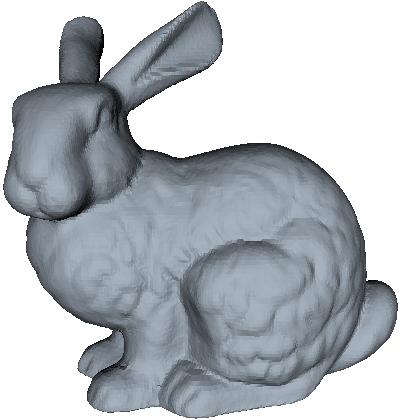
\includegraphics[width=2.6in]{images/ch2/bunny}
                \caption{original}
                \label{fig:bunnyOrig}
        \end{subfigure}%
        \begin{subfigure}[b]{2.6in}
                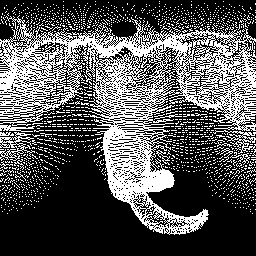
\includegraphics[width=2.6in]{images/ch2/spherical2DMap}
                \caption{transform}
                \label{fig:bunnySPTed}
        \end{subfigure}%
        \caption{The Spherical Map Transform.}
       \label{fig:smtExample}
\end{figure*}

\subsection{Projection-map transform}

The projection map transform is similar to an orthogonal projection of the volume along some given axis. For the projection map transform, given an output image $Im_a$ and an input volume $Vol_a$, each pixel in $Im_a$ is defined mathematically as the summation of values along a particular axis given the image coordinates. The x-axis transform and the z-axis transform are defined in equations \ref{eqn:xPMT} and \ref{eqn:zPMT} respectively. \\

\begin{equation} \label{eqn:xPMT}
Im(z,y) = \sum_{x=0}^{N}{Vol_a(x,y,z)}
\end{equation}

\begin{equation} \label{eqn:zPMT}
Im(x,y) = \sum_{z=0}^{N}{Vol_a(x,y,z)}
\end{equation}

The process defined by equation \ref{eqn:xPMT} maps 3D z-axis translation to 2D x-axis translation, whilst equation \ref{eqn:zPMT} maps 3D x-axis and y-axis translation into 2D x-axis and y-axis translation.


To assess the performance of our method, the size of the volumes being registered is defined as $N^3$ whilst each frame is sampled at a resolution of $W$ $\times$ $H$. The projection process requires $12WH$ operations whilst re-sampling the point cloud requires $2WH$ operations. The Volume Registration process, $VolumeRegister{\theta \varphi t_x t_y t_z}(V_1, V_2)$ consists of 2 $\times$ Hanning windowing processes, 2 $\times$ 3D FFTs, 2 $\times$ volume-logs, 2 $\times$ log-spherical transforms, 2 $\times$ phase correlation processes and 1 $\times$ linear transformation and peak finding. 

The Hanning windowing function requires 26 operations. The 3D FFT has complexity of $3N^3\log{N}$, the log and log-spherical transform functions require 3 and 58 operations per voxel respectively. Multiplying two frequency spectra together and transforming a volume requires 15 and 30 operations per voxel respectively. Finding the peak value requires $2N^3$ operations. The complexity in terms of number of operations for the phase correlation process is given in Eq. \ref{eqn:PCFULLPERFORMANCE} This process requires 2 $\times$ 3D FFTs, 1 $\times$ frequency spectra multiplication, and 1 $\times$ peak finding operation. 
\begin{equation} \label{eqn:PCFULLPERFORMANCE}
6N^3\log{N} + 2N^3 + 15
\end{equation}
The total complexity can then be found by taking into account the projection and re-sampling totals as well as the total for $VolumeRegister{\theta \varphi t_x t_y t_z}(V_1, V_2)$. Tallying the number of operations for each process and multiplying them by number of times the process is performed gives us the number of operations as a function of $W$, $H$ and $N$ in Eq. \ref{eqn:FULLPERFORMANCE}.
\begin{equation} \label{eqn:FULLPERFORMANCE}
6N^3 + 28WH + 18(N^3\log{N}) + 230
\end{equation}
\begin{figure*}[t] 
        \centering
        \begin{subfigure}[b]{2.0in}
                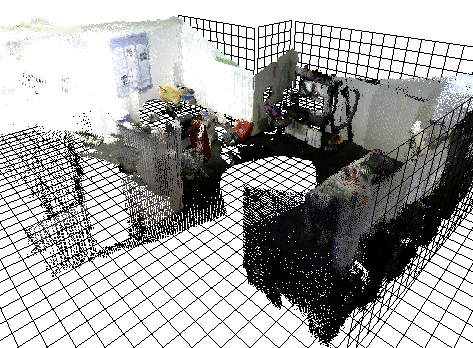
\includegraphics[width=2.0in]{images/ch2/unit21}
                \caption{Apartment}
                \label{fig:RECON_UNIT}
        \end{subfigure}%
        \begin{subfigure}[b]{2.0in}
                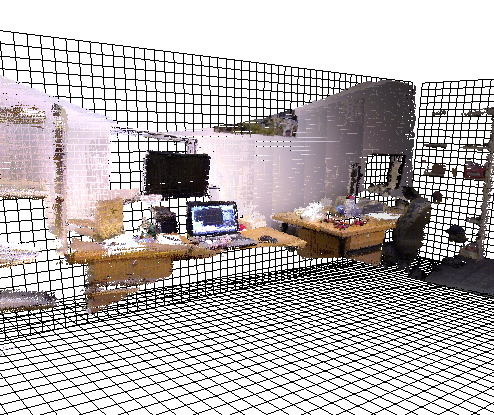
\includegraphics[width=2.0in]{images/ch2/officeA}
                \caption{Office}
                \label{fig:RECON_OFFICE}
        \end{subfigure}%
        \begin{subfigure}[b]{2.0in}
                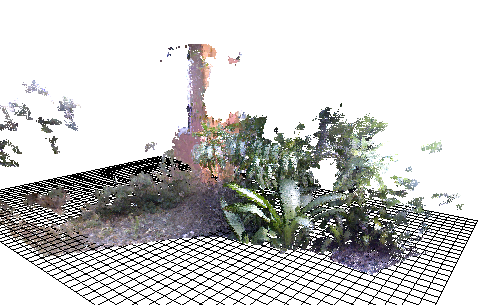
\includegraphics[width=2.0in]{images/ch2/outdoorA}
                \caption{Garden}
                \label{fig:RECON_GARDEN}
        \end{subfigure}
       \caption{Reconstructed Scenes.}
       \label{fig:RECONSTRUCTIONS}
\end{figure*}



To compare performance of the generic volume registration method with the speed up, we use the complexity defined in equation \ref{eqn:FULLPERFORMANCE}. Here, we ignore the cost of projecting the depth map. The 3D DFT has complexity $3N^3log(N)$. This is the first step (see figure \ref{fig:PIPELINE3}), the next is the spherical-map transform which is complexity $45N^3$. If processed on the GPU the performance becomes 45 operations per voxel assuming that one voxel is assigned to one unit of processing. A 3D transform is 30 operations per voxel, 2D phase correlation requires 15 operations to multiply the frequency spectra and $2N^2log(N)$ operations to do the 2D FFT. Finally a projection map transform requires 1 operation per voxel. \\

In total, the proposed method requires $2 \times$ 3D FFTs, $2 \times$ spherical-map transforms, $1 \times$ 3D geometrical transformation, $3 \times$ 2D phase correlations and $4 \times$ projection map transforms. The total complexity is added up for all of these functions and given in equation \ref{eqn:FULLPERF2}. \\

\begin{equation} \label{eqn:FULLPERF2}
6log(N)\times (N^3 + N^2) + 169
\end{equation}

Figure \ref{fig:perfComp} provides a visualization of the performance improvement which the proposed method achieves over the original Fourier volume registration approach. It is clear that the proposed method is around 3 times faster
than the original Fourier based volume registration approach. This is due to the reduction in the amount of data to process afforded by the novel spherical-map transform and orthogonal projection methods.

\begin{figure}[t]
\centering
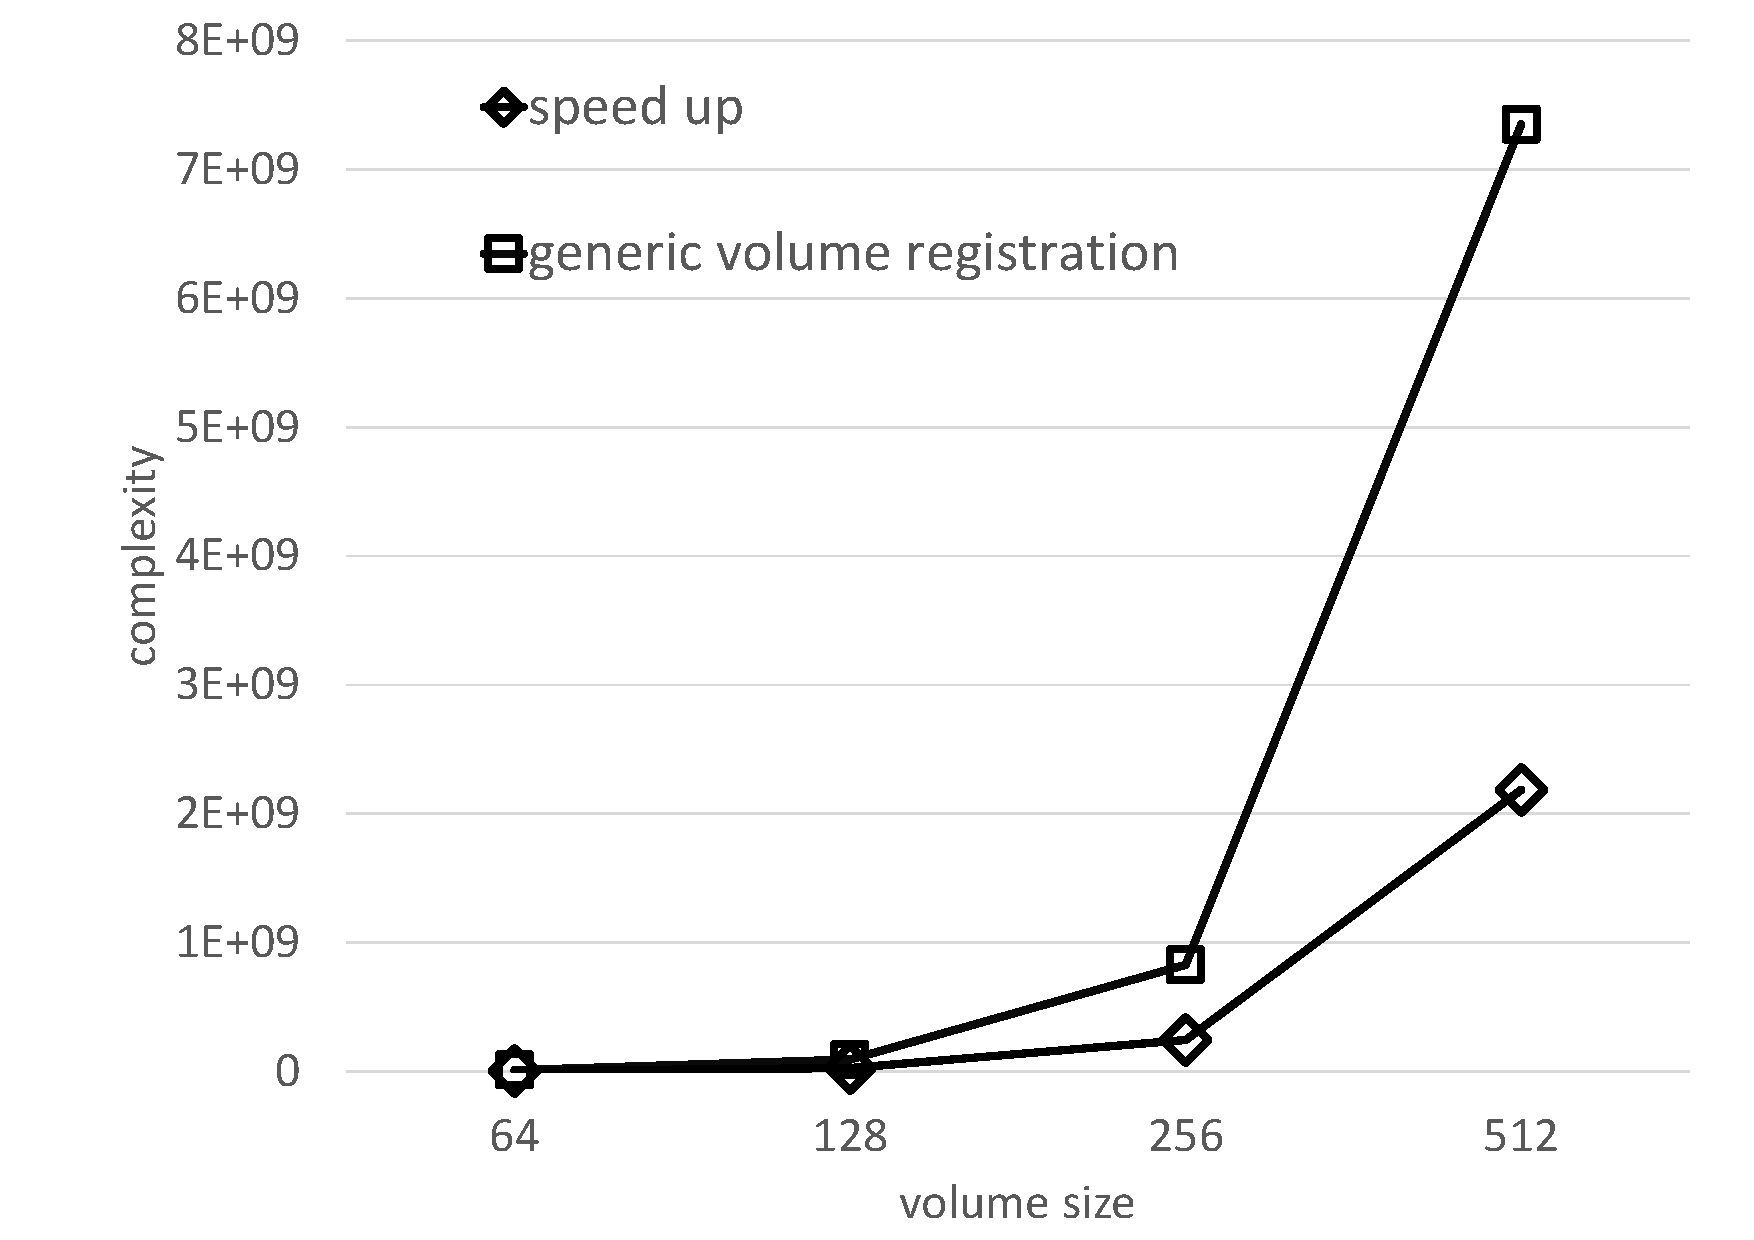
\includegraphics[width=3.0in]{images/ch2/perfcomp}
\caption{Comparison of performance between volume registration and the proposed speed up for different volume sizes.}
\label{fig:perfComp}
\end{figure}




\subsection{7-DoF Based Fourier Registration}

\section{3D Reconstruction Data Representation}

\subsection{3D ShadeTree Coding}

\subsection{PlaneTree Coding}

\section{Depth Sensor Based Reconstruction}

\label{METHOD_SECLL}
The proposed SLAM method consists of various steps. First each frame $f_i$ that is captured, consisting of a colour and depth image pair is projected into 3D space, forming colour point cloud $points_i$ and re-sampled into a volume $V_i$. Then, the transform parameters between pairs of volumes $V_i$ and $V_{i+1}$ are estimated using $VolumeRegister_{\theta \varphi t_x t_y t_z}$ shortened to $VR_{\theta \varphi t_x t_y t_z}$. These parameters are used to update transformation matrix $M$. The points corresponding to $f_2$ ($points_1$) are then transformed using the updated $M$ matrix and added to the cumulative $PointCloud$ database. Two lists, $Cameras$ and $Poses$, are also updated to track camera pose and location per frame. This basic procedure is given in listings \ref{algorithm:PCSLAM} and elaborated upon in subsequent subsections.
\begin{figure}
\begin{lstlisting}[language=c++,caption=Phase Correlation Based SLAM Algorithm,label=algorithm:PCSLAM,mathescape,basicstyle=\ttfamily]
$f_1$ = ReadFrame();
$PointCloud$ = project($f_1$);
$M$ = IdentityMatrix();
$Camera$ = $[0, 0, 0]^T$;
$Pose$ = $[0, 0, 1]^T$;
$Cameras$ = $\left[Camera\right]$, $Poses$ = $\left[Pose\right]$;
while(more frames){
	$f_2$ = ReadFrame();
	$points_1$ = project($f_2$);
	$points_2$ = project($f_1$);
	$V_1$ = ResampleVolume($points_1$);
	$V_2$ = ResampleVolume($points_2$);
	$(\theta, \varphi, t_x, t_y, t_z) = VR_{\theta \varphi t_x t_y t_z}(V_1, V_2)$;
	$M = M \times$TransformMat($(\theta, \varphi, t_x, t_y, t_z)$);
	$points_1$ = Transform($points_1$, $M$);
	$PointCloud$ = $PointCloud \cup points_1$;
	$Camera$ = $M^{-1} \times Camera$;
	$Pose$ = $M^{-1} \times Pose$;
	$Cameras.add(Camera)$;
	$Poses.add\left(\frac{Pose-Camera}{|Pose-Camera|}\right)$;
	$f_1$ = $f_2$;
}
\end{lstlisting}
\end{figure}
\subsection{Sensor Input}
The input to our method is a color and depth image pair, $f(u,v)$ and $g(u,v)$ obtained using an Asus Xtion PRO LIVE sensor at a resolution of $640 \times 480$. Each pixel is projected into 3D space using $X_{u,v} = \frac{(u - c_x)Z_{u,v}}{f}$, $Y_{u,v} = \frac{(v - c_y)Z_{u,v}}{f}$ and $Z_{u,v}$ = $g(u,v)$. 
Here, $[c_x c_y]^T$ represent the center of the image whilst $f$ represents the focal length, defined as $525.0$. The point clouds generated by projecting these images are then quantized into image volumes. Results reported in this paper were obtained using volumes of $384^3$ voxels in size.
\begin{figure*}[t]
\centering
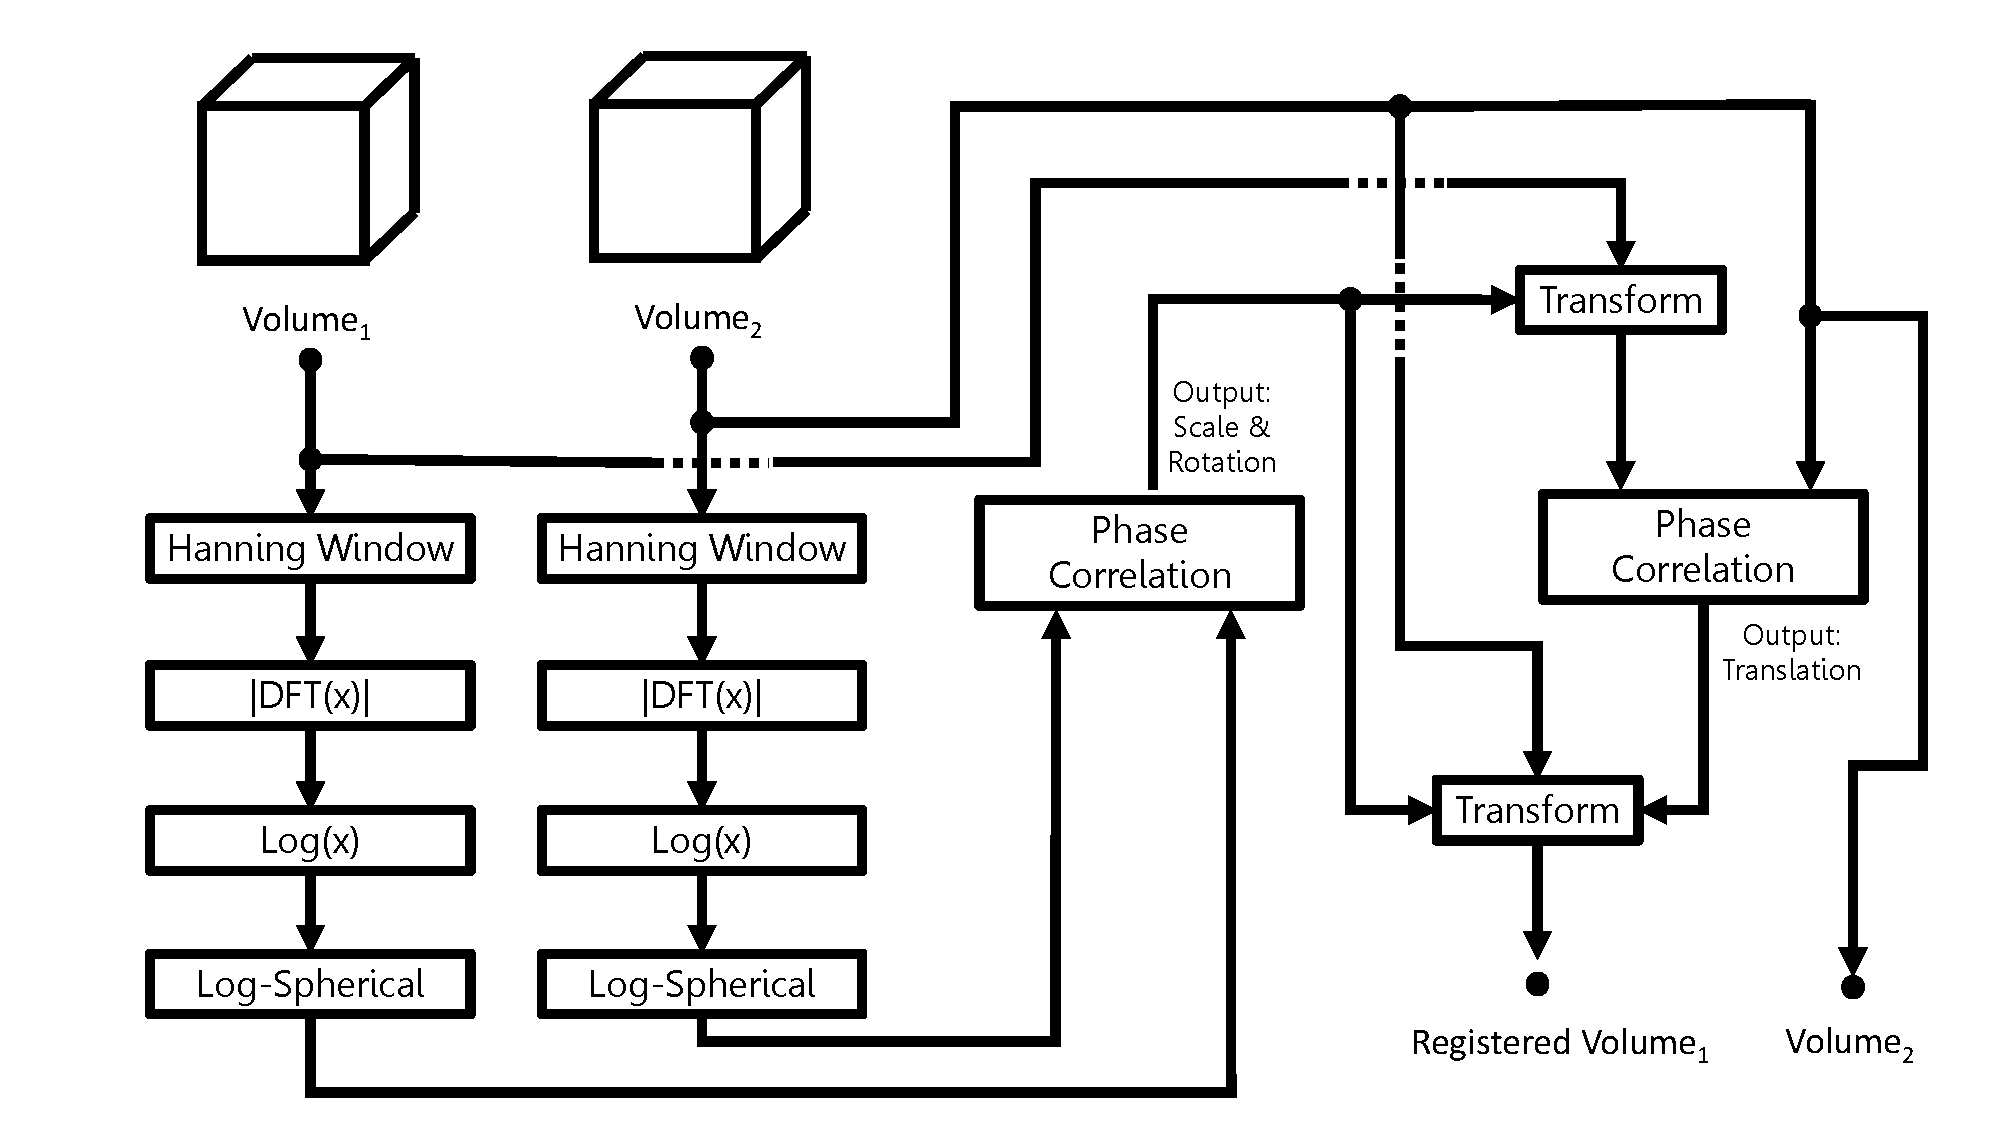
\includegraphics[width=6.0in]{images/ch2/pipeline2}
\caption{System Diagram for Registration Process}
\label{fig:PIPELINE}
\end{figure*}


\section{Stereo Camera Based Reconstruction}

\section{Monocular Sensor Based 3D Reconstruction}



\section{Conclusion} % Methodology
%\begin{savequote}[8cm]
  ``I just wondered how things were put together.''
  \qauthor{Claude Shannon}
\end{savequote}
\makeatletter
\chapter{Experiments and Results}

\section{Experiments}

This section discusses the types of experiments performed. First, a survey on codec evaluation and comparison techniques is presented, then those techniques used to evaluate the SOT are reported. Next, the experiment environment used is discussed, along with the data set used in experiments.

\begin{figure*}[t] 
        \centering
        \begin{subfigure}[b]{2.0in}
                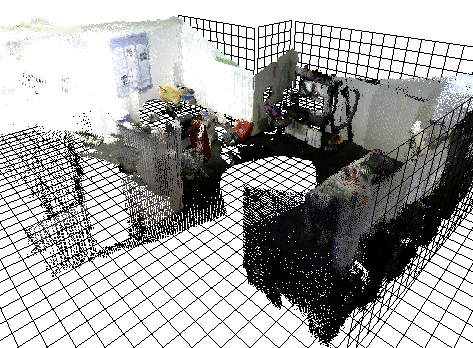
\includegraphics[width=2.0in]{images/ch2/unit21}
                \caption{Apartment}
                \label{fig:RECON_UNIT}
        \end{subfigure}%
        \begin{subfigure}[b]{2.0in}
                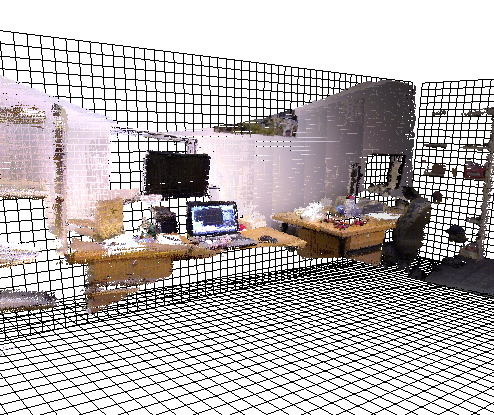
\includegraphics[width=2.0in]{images/ch2/officeA}
                \caption{Office}
                \label{fig:RECON_OFFICE}
        \end{subfigure}%
        \begin{subfigure}[b]{2.0in}
                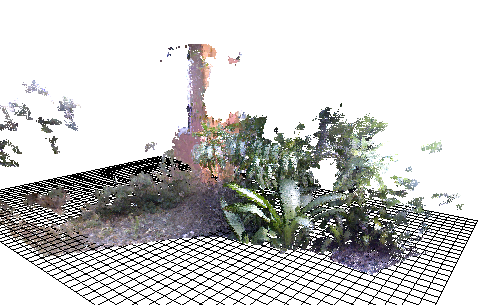
\includegraphics[width=2.0in]{images/ch2/outdoorA}
                \caption{Garden}
                \label{fig:RECON_GARDEN}
        \end{subfigure}
       \caption{Reconstructed Scenes.}
       \label{fig:RECONSTRUCTIONS}
\end{figure*}


\subsection{Codec Evaluation \& Comparison Techniques}

Codec evaluation involves comparing storage requirements between the original model and codec output. In the case of lossy codecs, a quantitative quality metric is also required. Compression metrics are easy to compute, quality metrics are more involved and there have been many proposed techniques. Quality metrics compare the distortion created by the codec relative to the original model. Two measurements are usually performed, the distance from the compressed model to the original and the distance from the original to the compressed model. Quality metrics are split into empirical and perceptual based metrics. Empirical metrics measure geometric error and perceptual metrics estimate human perception. Perception based metrics are a part of psychophysics research. For a more in-depth survey of these methods, see work by Bubill \textit{et al.} \cite{Bulbul11Assessing}.

\subsubsection{Compression Metrics}

In the context of 3D model compression, the file size of both, the compressed model and the original are compared. Alternatively, the file size of the compressed model from one codec can be compared to the file size of the same model compressed using another codec. The compression ratio ($CR$), defined as the original file size divided by the compressed file size, is a measure of compression performance. Another metric used is called the bit rate, different bit rates are used depending on the representation being compressed. The mesh representation uses bits per vertex (bpv) and bits per triangle (bpt), the volumetric representation uses bits per voxel and the point cloud representation uses bits per point.

\subsubsection{Empirical Error Metrics}

The following metrics are used to assess the error between two data samples. For two points, $p$ \& $q$, in $\Re^3$ space, the basic euclidean distance metric,
$$
ED(q,p) = \sqrt{(q_x - p_x)^2 + (q_y - p_y)^2 + (q_z - p_z)^2}
$$,
the absolute error,
$$
AE(q,p) = \|q_x - p_x\| + \|q_y - p_y\| + \|q_z - p_z\|
$$
and the squared error $SE$, 
$$
SE(q,p) = (q_x - p_x)^2 + (q_y - p_y)^2 + (q_z - p_z)^2
$$
are often used as a basis for other metrics. 3D models can be sampled into a set of points in $\Re^3$. Using these samples, the following metrics can be used: sum of distances ($SOD$), sum of absolute differences ($SAD$), sum of squared errors ($SSE$), mean square error ($MSE$) and root mean square error ($RMS$). Since the two models may be sampled differently, the minimum error from one sample to the others is used. These metrics are defined below using two point sets, $A$ \& $B$ where the length of these sets is $M$ and $N$ respectively.
$$
SOD(A,B) = \sum_{k=0}^{M} \min_{b \in B}(ED(A_k,b))
$$

$$
SAD(A,B) = \sum_{k=0}^{M} \min_{b \in B}(AE(A_k,b))
$$

$$
SSE(A,B) = \sum_{k=0}^{M} \min_{b \in B}(SE(A_k,b))
$$

$$
MSE(A,B) = \frac{1}{M}SSE(A,B)
$$

$$
RMS(A,B) = \sqrt{MSE(A,B)}
$$

For each of these metrics, $METRIC(A,B) \neq METRIC(B,A)$. Therefore, these methods are often averaged (below). This is termed the average metric (AM), as opposed to the minimum metric (MM) which is the smallest value of the two.

$$
AvgError = \frac{Metric(A,B)+Metric(B,A)}{2}
$$

Another metric, the Hausdorff distance ($HD$) is a measure of overall shape similarity. It is defined as the largest value of the maximum distances between objects from $A$ to $B$ and from $B$ to $A$. For example, for two objects $A$ \& $B$, the Hausforff distance $HD$, from $A$ to $B$, is defined as,
$$
HD(A,B) = \max(D(A,B),D(B,A))
$$
where $D(A,B)$ is defined as,
$$
D(A,B) = \{a \in A \| \max(dist(a,B)\}
$$
and $dist(a,B)$ is defined below.
$$
dist(a,B) = \{b \in B \left| \min(\|a-b\|)\right.\}
$$

\subsubsection{Human Perception Based Metrics}

Lavoue \textit{et al.} \cite{Lavoue06Perceptually} devised a metric based on structural distortion, this method correlates well with human perception. It is based on the SSIM method of Wang \textit{et al.} \cite{Wang04Image}, which is a popular image metric. Lavoue \textit{et al.} call their method the, Mesh Structural Distortion Measure (MSDM). An updated version of this metric was also developed \cite{Lavoue11Multiscale}.

\paragraph{Laplacian Metric}

Karni \& Gotsman \cite{Karni00Spectral} developed their own on-line metric for use during their spectral based codec. It is based on the laplacian and measures the difference between two objects in terms of their smoothness. 

\paragraph{Elastic Deformation Based Metric}

Bian \textit{et al.} \cite{Bian09Evaluation} developed a novel metric, useful for both on and off-line model comparison. The algorithm is based on the theory of strain fields. A strain field is a metric derived from elasticity, it is used to describe the deformation of some object which has elastic properties. Using this concept, both models are treated as having elastic properties in order to perform quality assessment.

\paragraph{Saliency Based Metrics}

Howlett \textit{et al.} \cite{Howlett04Experimental} and Lee \textit{et al.} \cite{Lee05Mesh} both presented work aimed at determining salient features in 3D models. They incorporated these findings in their own metrics. Howlett \textit{et al.} used a human gaze detection device to study the psychophysical effects of viewing 3D objects. Both of these metrics are based on preserving the sections of the object in which any distortion would be visibly noticeable to humans.

\paragraph{The Depth Difference Metric}

Krivokuca \textit{et al.} \cite{Krivokuca12New} developed a perceptual based metric for the off-line quality assessment of 3D models. This method is independent of model representation and is based on generating multiple depth maps from different orthographic perspectives. It improves upon both the Hausdorff distance and RMS error and is good at detecting both small and large geometric errors. Krivokuca \textit{et al.} call their method, the Depth Difference (DD). It works by comparing orthographic depth maps from both the original and compressed models. First a difference depth image is calculated ($DDI$) from orthographic depth maps of the original object ($DIO$) and of the compressed object ($DIC$). The $DDI$ is calculated using element-wise matrix subtraction,

$$
DDI = DIO - DIC
$$

Then the average depth distance value ($ADD$) is calculated from the $DDI$ matrix, this equation is presented below.

$$
ADD = \frac{1}{MN} \sum_{y=0}^{M} \sum_{x=0}^{N} DDI_{y,x}
$$

This $ADD$ value is then summed up and averaged over different orthographic views, this average is the Depth Difference.

\subsection{Codec Performance Assessment}

The experiments performed use a number of different metrics to quantify the performance of the SOT and compare it with other codecs. The quality metrics used include: mean distance, $RMS$, Depth Difference ($DD$), $MSE$, and qualitative perception. Most research uses the $MSE$ and $RMS$ because they are simple and provide an accurate measurement of quality. Since the data which the SOT is manipulating was designed for human visual consumption, the perceptual metric, DD is used. Our implementation of the DD metric uses five orthogonal projections corresponding to the sides of a cube (excluding the bottom face). Qualitative comparisons are also used to provide insight into the visual quality of the models which the SOT produces. The storage metrics used include: number of bytes and bpv. Bits per vertex is used most often because the input and output of the SOT is a polygonal mesh, and because it is widely used in the literature as part of rate-distortion graphs.

Results provided for the OT use the MM and results for the SOT use the AM. This is because the SOT can represent both outside and inside views of the mesh, whilst the OT can only represents the outside view. All measurements are computed using a $512 \times 512 \times 512$ bounding box, but when comparing the SOT with other codecs, the error is converted to the same bounding box used by the other codec.

\subsubsection{The Metro Program}

In order to ensure the accuracy of geometric errors, the Metro software tool is used to independently assess the quality of models produced by the SOT. This tool takes two models as input and produces the forward and backward $RMS$, mean distance and Hausdorff distance between the two. Metro Version 4.06 was used in all experiments, details about this software can be found in work by Cignoni \textit{et al.} \cite{Cignoni98Metro}.

\subsection{Experiment Environment}

All experiments were performed on an ASUS computer with an Intel i5 CPU and 4 GB of RAM, this machine was running Windows 7. The SOT and OT were written in C++ using Microsoft's Visual Studio IDE, and OpenGL was used to provide visualizations of all models.

\subsection{Data Set}

Industry standard models are used to evaluate the SOT. Six widely used 3D models are used in experiments. These models contain relatively large amounts of geometric information making them a challenge for compression. Figure \ref{dataset} presents this data set. For each model the name, vertex and triangle count are given. With the exclusion of the ball model, these models are commonly used in compression and simplification research. This data set was obtained from the Georgia Institute of Technology's Large Geometric Models Archive \cite{LargeGeometricModelsArchive}. The ball model is included in experiments to provide insight into the compression of smaller 3D models. 


\subsection{Shade-Octree Experiments}

Some experiments are performed on the SOT for the sole purpose of evaluating the best LOD and distance code search length (DCL) to use. Since these variables directly affect he SOT's efficiency, experiment results are provided. Both of these experiment types are described in detail below.


\subsubsection{Distance Code Length Tests}

The SOT makes use of four distance codes per node. These distance codes are truncated to a multiple of the node's region size. This multiple is called the distance code length (DCL). To evaluate the optimal DCL, six sets of experiments are performed, each using DCL values ranging from one to six. For each experiment, $MSE$ threshold values of: $1$, $16$ and $512$ are used, these provide rate-distortion curves for each DCL experiment. In these experiments, the bunny model is used and both visual and graphical results are presented. This test is important because it reveals the best choice for the DCL. The optimal selection of the DCL may have an impact on codec efficiency. 

\subsubsection{Maximum Level of Depth Tests}

The level of depth (LOD) threshold represents the minimum leaf region size (how far the tree can be decomposed). A smaller LOD provides more accuracy but requires more storage size, a larger code results in a smaller file size with more distortion. To select the best LOD, five experiments are performed using LOD values of: 1, 2, 4, 8 and 16. All results are obtained using the bunny model and both numerical and graphical results are provided. These experiments are performed to find the optimal choice of the LOD threshold, which affects the efficiency of the SOT. 

\subsection{Codec Comparisons}

The SOT is compared with a generic implementation of the OT, as well as other state of the art codecs. These experiments are discussed in the sections below.


\subsubsection{OT Comparison}

The OT algorithm is the main competitor of the SOT, it is a very well known and used 3D compression and representation structure. Rate-distortion curves are used to compare these codecs. In these experiments, $bpv$ is used as the bit rate, and both $DD$ and the $MSE$ metrics are used to measure quality. A qualitative quality analysis is also used to compare the two codecs. 

\subsubsection{State of the Art Comparisons}

The SOT is compared to other codecs which have been shown to have state of the art performance. The method by Peng \& Kuo \cite{Peng05Geometry-Guided} is compared with the SOT using a rate-distortion graph with the rabbit model. The progressive wavelet compression method by Khodakovsky \textit{et al.} \cite{Khodakovsky00Progressive} is also compared using a rate-distortion graph using the bunny model. Both the spectral codec by Karni \& Gotsman \cite{Karni00Spectral} and the state of the art single-rate codec by Touma \& Gotsman \cite{touma98triangle} are compared using a qualitative quality assessment of the bunny model. The hierarchical point-cloud codec by Siddiqui \textit{et al.} \cite{Siddiqui07Octree} is also compared with the SOT using a qualitative analysis. Recent state of the art codecs, including the FOLProM codec by Peng \textit{et al.} \cite{Peng10Feature} and the spectral codec by Bayazit \textit{et al.} \cite{Bayazit103DMesh} are also compared.
 % Experiments &
%\section{Results}

This section presents and analyses the results from experiments. The experiments used to evaluate the optimal LOD and DCL values are presented first. Then the SOT is compared with the OT codec and with the current state of the art codecs from the literature. Results include both, rate-distortion and qualitative quality tests. 

\subsection{LOD \& DCL Evaluation}

\subsubsection{Distance Code Length Evaluation}

DCL values tested include $1$, $2$, $3$, $4$, $5$ and $6$. First, rate-distortion graphs are presented, then visual results are discussed.

\paragraph{Rate-Distortion Graphs}

Figure \ref{DistanceCodeRDGraphs} shows the rate-distortion graphs used to evaluate the different DCL values. The graphs in the top row use the $MSE$ metric and the graphs in the bottom row use the depth difference ($DD$) metric. The $MSE$ rate-distortion graphs suggest that DCL values of $5$ and $6$ perform slightly better than the others. The $DD$ rate-distortion graphs show that DCL values of $6$ and $3$ perform better, with $6$ performing well at high bit rates and $3$ performing well at lower to mid level bit rates. Overall, these results do not provide a clear indication of an optimal DCL value but it can be seen that values of $1$ and $2$ do not perform as well as the higher values.


\paragraph{Visual Comparisons}


Two sets of visual comparisons are presented to evaluate the optimal DCL value. Figure \ref{DistanceCodeVisualTests1} shows results at higher bit rates and figure \ref{DistanceCodeVisualTests2} shows results at lower bit rates. Both sets of results suggest that a DCL value of $1$ produces undesirable models with many holes. Results seem to be quite similar for DCL values of $3$ and above. A DCL value of $2$ provides a slight $MSE$ advantage at a higher bit cost, but in both figures, this quality difference is not noticeable.


\paragraph{Conclusion}

Results shown that a DCL value of $1$ produces poor results, both in a rate-distortion and qualitative quality sense. A DCL value of $2$ produces a higher calibre model in the $MSE$ sense, at the expense of a higher bit rate. This $MSE$ quality advantage is unnoticeable in qualitative comparisons, compared to values of $3$ and above. Therefore it is generalized that, DCL values of $3$ and above, are the best choice for use in the SOT.

\subsubsection{Level of Depth Threshold Evaluation}

LOD tests are used to evaluate the optimal choice of LOD threshold. Different LOD threshold comparisons include: $1$, $2$, $4$, $8$ and $16$.

\paragraph{Rate-Distortion Graphs}

Figure \ref{LevelsOfDepthRDGraphs} shows two rate-distortion graphs, the left graph uses the $MSE$ metric and the right graph uses the perceptual $DD$ metric. The $MSE$ graph suggests that an LOD threshold value of $8$ is optimal for higher bit rates and a value of $16$ is best for lower bit rate compression. The $DD$ metric graph suggests that the LOD of $8$ is the optimal threshold value. It produces the best results and is comparable to LOD $16$ even at low bit rates. Both graphs suggest that LOD values of $1$ and $2$ result in poor performance, this is due to the fact that these levels require more branches in the tree, increasing storage requirements. An SOT with a shallow tree that accurately accurately approximates the model is ideal.

\paragraph{Visual Comparisons}


Visual comparisons further provide an indication of the best LOD threshold to use. Figure \ref{LevelsOfDepthVisualTests1} shows high bit rate results using different LOD values, and figure \ref{LevelsOfDepthVisualTests2} shows the same tests for lower bit rates. In figure \ref{LevelsOfDepthVisualTests1}, the bit rate becomes lower and lower as the LOD value is raised, but only on the transition from $8$ to $16$ does this advantage wear off, as the LOD $16$ model is more distorted than the rest. This further suggests that the optimal LOD value is $8$. Figure \ref{LevelsOfDepthVisualTests2} also suggests this conclusion. Notice that with low bit rate compression, the models with LOD values ranging $1-8$ look similar, but $8$ has the lowest bit rate.


\paragraph{Conclusion}

The optimal LOD value is more obvious than the optimal DCL code. Both, rate-distortion graphs and visual results reveal that the optimal LOD threshold is level $8$. Since all models are bound to a $512\times 512 \times 512$ box, where the root node is defined as level $0$, the SOT should be decomposed until a maximum tree depth of $6$.

\subsection{SOT vs. OT Results}

This section presents results comparing the the SOT with the OT. Models tested include: Ball, Bunny, Horse, Rabbit, Dragon, Angel and Happy Buddha. Tabulated results for the SOT are provided in Appendix \ref{AppendixA}.

\subsubsection{Rate-Distortion Graphs}

RD results for the ball model are presented in figure \ref{ballRDGraphs}. The $MSE$ metric graph (left) shows that the SOT outperforms the OT codec, and the $DD$ metric graph supports this conclusion. In the $DD$ graph, the OT cannot reach the quality of the SOT, even at very high bit rates.

Rate-distortion results for the bunny model are presented in figure \ref{bunnyRDGraphs}. These results are similar with those obtained using the ball model. In these results, the SOT outperforms the OT codec. In the rate-distortion graphs for the horse, the $MSE$ metric graph on the left of figure \ref{horseRDGraphs} shows that the OT comes close to the performance of the SOT, but still has worse performance. When considering the same figure where the $DD$ metric is used (right), the SOT produces much better results than the OT.

Rate-distortion graphs for the: rabbit, angel, dragon and happy buddha are shown in figures: \ref{rabbitRDGraphs}, \ref{angelRDGraphs}, \ref{dragonRDGraphs} and \ref{happyRDGraphs} respectively. These results show similar findings in that the SOT is more efficient than the OT codec in terms of rate-distortion, especially in terms of quantitative perceptual quality (DD).

\subsubsection{Visual comparisons}

Visual comparisons make a case for the practicality of the SOT because this data is meant for human visual consumption. In figure \ref{ballVisualResults} the ball is coded with the SOT and OT, the outputs of these codecs are compared with the original model. These results show a large difference in quality between the SOT and the OT. The OT codec produces a blocky, spikey shape which does not correlate with the outline of the original model. The SOT produces a more visually pleasing result whilst using two thirds of the storage requirements of the OT. 


The bunny visual results are shown in figure \ref{bunnyVisualResults}, these results show that for a similar bit rate, the SOT codec produces a higher quality model than the OT. The outline of the SOT coded model looks similar to the original model, but does have some holes. The holes are present because the SOT is rendered directly from the tree structure without being filtered. Despite this, it is still less distorted than the model compressed using the OT. 


Visual results for the horse model are presented in figure \ref{horseVisualResults}. These results show that for a lower bit rate, the SOT codec produces a higher quality model compared with the OT. Results for the rabbit (figure \ref{rabbitVisualResults}) also show that for a lower bit rate, the SOT produces better quality models. In the rabbit results, the SOT coded model looks very similar to the original model whilst the OT coded model is blocky and distorted. It is clear that the OT has suffered from 3D aliasing. 

Visual results for the angel, dragon and happy buddha are provided in figures, \ref{angelVisualResults}, \ref{dragonVisualResults} and \ref{happyVisualResults} respectively. These results show that, at low bit rates, the SOT produces models which fit the outline of the original model better.


\subsubsection{Conclusion}

Results show that the SOT outperforms the OT codec in both, rate-distortion tests and in qualitatively quality analysis. The SOT produces models which match the general shape of the original model well, however some filtering is required to fill infrequently occurring holes. The OT produces models which have aliasing and distortion, plus the OT produces higher bit rates.

\subsection{Comparisons with the State of the Art}

Codecs used for state of the art comparisons include: the progressive mesh OT by Peng \textit{et al.} \cite{Peng05Geometry-Guided}, the wavelet codec by Khodakovsky \textit{et al.} \cite{Khodakovsky00Progressive}, FOLProM by Peng \textit{et al.} \cite{Peng10Feature}, the hierarchical point cloud codec by Siddiqui \textit{et al.} \cite{Siddiqui07Octree}, the valence driven codec \cite{touma98triangle}, the spectral codec by Karni \& Gotsman \textit{et al.} \cite{Karni00Spectral} and the other spectral codec by Bayazit \textit{et al.} \cite{Bayazit103DMesh}. 

\subsubsection{Rate-Distortion Graphs}

Figure \ref{Peng05Geometry-GuidedRDGraph} shows a rate-distortion graph comparing the progressive OT codec by Peng et al. \cite{Peng05Geometry-Guided} with the SOT.  Results show that the SOT outperforms this codec. Results comparing the SOT and the wavelet codec by Khodakovsky \textit{et al.} \cite{Khodakovsky00Progressive} are shown in figure \ref{Khodakovsky00ProgressiveRDGraph}. This graph uses the $MSE$ as the quality metric and the bunny model as codec input. This graph shows that the SOT outperforms the wavelet codec.


Peng \textit{et al.} have another, more recent codec called FOLProM  \cite{Peng10Feature}. Results are shown in figure \ref{Peng10FeatureRDGraph}. The left graph shows results for the dragon, and the right graph shows results for the rabbit model. In both graphs, the SOT has a better rate-distortion curve.

\subsubsection{Visual comparisons}

Figure \ref{SOTSiddiqui07OctreeVisualResults} shows visual results for the SOT and the codec by Siddiqui \textit{et al.} \cite{Siddiqui07Octree}. The two models on the left were compressed by the SOT, the middle model is the original and the models on the right were compressed by the point cloud OT codec. Results show that the SOT requires $2.840$ bpv to represent the original bunny model accurately, whilst the codec by Siddiqui \textit{et al.} requires at least $11.2$ bpv to to store the model at a similar quality level. At $8.3$ bpv their models become slightly distorted, and at $5.8$ bpv, they become very distorted, not reaching the quality of the SOT codec.
 

Figure \ref{SOTtouma98triangleKarni00SpectralVisualResults} shows visual results for the SOT, the valence driven approach \cite{touma98triangle} and the spectral codec \cite{Karni00Spectral}. The first two models are SOT outputs, the center model is the original bunny model, the center right model was produced by the spectral codec and the far right model was compressed using the valence driven approach. The SOT coded models look quite similar to the original model, the SOT model with a bit rate of $1.461$ does look a bit blocky, however it has a much lower bit rate compared with the other models. The far left codec with a bit rate of $3.984$ is similar to the original model but suffers from a missing patch on its left foot, however, the ears and legs correlate well with the original model. The valence driven codec produces undesirable results, its output model is lumpy and is quite distorted. The spectral coded model looks better but looks overly lumpy. The SOT's improvement over the spectral codec is somewhat arguable, but the SOT is a clear improvement over the valence driven approach.


Figure \ref{SOTBayazit103DMeshVisualResults} shows results comparing the SOT with the recent spectral codec by Bayazit \textit{et al.} \cite{Bayazit103DMesh}. At a bit rate of $1.461$, the SOT codec produces a smoother version of the original model, whilst the spectral codec by Bayazit requires $2.523$ bpv to produce a model which is very lumpy and distorted. These results suggest the SOT is the better codec.

\subsection{Conclusion}

Experiments show that the optimal LOD threshold is $8$ and the best DCL values are above or equal to $3$. Results have also revealed that the SOT outperforms both the OT and other state of the art codecs from the literature in terms of rate-distortion and qualitative quality. The hierarchical SOT method produces models which accurately reflect the general shape of the original model and transform based codecs produce models which are lumpy. These results suggest that the SOT is among the current state of the art 3D data compression schemes available.

 % Results
%\begin{savequote}[8cm]
  ``Learn from yesterday, live for today, hope for tomorrow. The important thing is not to stop questioning.''
  \qauthor{Albert Einstein}
\end{savequote}
\makeatletter
\chapter{Conclusion}

\section{Research Aims Revisited}

The primary aim of this research was to improve the storage, quantitative quality and perceptual quality of 3D models. Hierarchical methods were investigated and this led to a new image codec, ILQT \cite{Lincoln13Interpolating} as well as the proposed scheme, the Shade-Octree. The research question was, ``Do hierarchical techniques bring state of the art compression performance to 3D data?'' Results from chapter 4 show that the SOT outperforms the OT compression scheme as well as several state of the art methods in terms of rate-distortion and perceptual quality. The primary aim of this research has been accomplished because the SOT produces models which have improved storage efficiency, whilst improving quantitative quality and perceptual quality compared with other compression schemes. The proposed research question can also be answered. The SOT, a hierarchical codec, does achieve state of the art performance in the field of 3D data compression.

\section{Future Work}

There is still much work to be done in the area of hierarchical 3D data compression. One possible project could be to improve the SOT. Currently the SOT can produce holes in the output mesh, an investigation of this may lead to improved results. Other projects could investigate the extension of the PJQ, wedglet, BSP-tree and QB tree to 3D model compression.
 % Conclusion
\appendix
none
%\makeatletter
\chapter{Appendix A}
\label{AppendixA}

\section{Tabulated Results}

\begin{table}[h]
\begin{tabular}[c]{|c|c|c|c|c|c|c|c|c|}
\hline\multicolumn{9}{|c|}{\textbf{SOT Results Using the Ball Graph}}\\
\hline
\textbf{Threshold} & \textbf{LOD} & \textbf{bytes} & \textbf{Mean} & \textbf{RMS} & \textbf{MSE} & \textbf{DD} & \textbf{Hausdorff} & \textbf{bpv}\\
\hline
1 & 8 & 2877 & 0.209 & 0.335 & 0.112 & 1.186 & 9.938 & 47.751\\
\hline
2 & 8 & 2111 & 0.309 & 0.473 & 0.223 & 1.603 & 8.899 & 35.037\\
\hline
4 & 8 & 1517 & 0.448 & 0.657 & 0.432 & 2.287 & 8.269 & 25.178\\
\hline
8 & 8 & 1111 & 0.603 & 0.917 & 0.841 & 4.846 & 21.755 & 18.440\\
\hline
16 & 8 & 928 & 0.674 & 1.036 & 1.073 & 6.052 & 21.755 & 15.402\\
\hline
32 & 8 & 841 & 0.741 & 1.270 & 1.613 & 11.391 & 21.755 & 13.959\\
\hline
64 & 8 & 856 & 0.743 & 1.275 & 1.626 & 11.526 & 21.755 & 14.207\\
\hline
\end{tabular}
\caption{A table displaying results for the SOT using the Ball model}
\label{table:SOTTableBall}
\end{table}

\begin{table}[h]
\begin{tabular}[c]{|c|c|c|c|c|c|c|c|c|}
\hline\multicolumn{9}{|c|}{\textbf{SOT Results Using the Bunny Graph}}\\
\hline
\textbf{Threshold} & \textbf{LOD} & \textbf{bytes} & \textbf{Mean} & \textbf{RMS} & \textbf{MSE} & \textbf{DD} & \textbf{Hausdorff} & \textbf{bpv}\\
\hline
1 & 8 & 6566 & 0.376 & 0.609 & 0.371 & 2.814 & 10.081 & 1.461\\
\hline
2 & 8 & 5475 & 0.482 & 0.744 & 0.554 & 3.005 & 11.532 & 1.218\\
\hline
4 & 8 & 4415 & 0.622 & 0.914 & 0.836 & 3.468 & 11.777 & 0.983\\
\hline
8 & 8 & 3632 & 0.809 & 1.172 & 1.374 & 3.946 & 14.448 & 0.808\\
\hline
16 & 8 & 2945 & 1.061 & 1.513 & 2.290 & 4.805 & 21.251 & 0.655\\
\hline
128 & 8 & 2096 & 1.514 & 2.162 & 4.674 & 7.291 & 21.283 & 0.466\\
\hline
256 & 8 & 1984 & 1.603 & 2.311 & 5.343 & 8.270 & 23.680 & 0.442\\
\hline
512 & 8 & 1878 & 1.673 & 2.442 & 5.964 & 9.163 & 23.680 & 0.418\\
\hline
\end{tabular}
\caption{A table displaying results for the SOT using the Bunny model}
\label{table:SOTTableBunny}
\end{table}

\begin{table}[h]
\begin{tabular}[c]{|c|c|c|c|c|c|c|c|c|}
\hline\multicolumn{9}{|c|}{\textbf{SOT Results Using the Horse Graph}}\\
\hline
\textbf{Threshold} & \textbf{LOD} & \textbf{bytes} & \textbf{Mean} & \textbf{RMS} & \textbf{MSE} & \textbf{DD} & \textbf{Hausdorff} & \textbf{bpv}\\
\hline
1 & 8 & 3349 & 0.469 & 0.731 & 0.534 & 2.778 & 9.523 & 0.553\\
\hline
2 & 8 & 3002 & 0.535 & 0.797 & 0.635 & 2.849 & 9.523 & 0.495\\
\hline
4 & 8 & 2605 & 0.676 & 0.986 & 0.972 & 3.132 & 13.978 & 0.430\\
\hline
8 & 8 & 2218 & 0.886 & 1.251 & 1.564 & 3.416 & 13.978 & 0.366\\
\hline
16 & 8 & 1949 & 1.121 & 1.560 & 2.433 & 4.002 & 16.394 & 0.322\\
\hline
128 & 8 & 1585 & 1.571 & 2.222 & 4.938 & 4.744 & 17.055 & 0.262\\
\hline
256 & 8 & 1516 & 1.669 & 2.385 & 5.689 & 4.922 & 17.055 & 0.250\\
\hline
512 & 8 & 1489 & 1.696 & 2.433 & 5.918 & 5.173 & 17.202 & 0.246\\
\hline
1024 & 8 & 1480 & 1.793 & 2.707 & 7.330 & 5.260 & 27.590 & 0.244\\
\hline
\end{tabular}
\caption{A table displaying results for the SOT using the Horse model}
\label{table:SOTTableHorse}
\end{table}

\begin{table}[h]
\begin{tabular}[c]{|c|c|c|c|c|c|c|c|c|}
\hline\multicolumn{9}{|c|}{\textbf{SOT Results Using the Rabbit Graph}}\\
\hline
\textbf{Threshold} & \textbf{LOD} & \textbf{bytes} & \textbf{Mean} & \textbf{RMS} & \textbf{MSE} & \textbf{DD} & \textbf{Hausdorff} & \textbf{bpv}\\
\hline
1 & 8 & 3041 & 0.389 & 0.572 & 0.327 & 1.405 & 9.438 & 0.363\\
\hline
2 & 8 & 2491 & 0.507 & 0.725 & 0.526 & 1.539 & 9.282 & 0.297\\
\hline
4 & 8 & 2017 & 0.681 & 0.942 & 0.888 & 1.908 & 9.282 & 0.241\\
\hline
8 & 8 & 1592 & 0.901 & 1.225 & 1.501 & 2.225 & 12.738 & 0.190\\
\hline
16 & 8 & 1226 & 1.156 & 1.536 & 2.359 & 2.687 & 12.831 & 0.146\\
\hline
128 & 8 & 810 & 1.680 & 2.275 & 5.176 & 3.684 & 18.271 & 0.097\\
\hline
256 & 8 & 763 & 1.757 & 2.409 & 5.802 & 4.044 & 18.271 & 0.091\\
\hline
512 & 8 & 737 & 1.809 & 2.520 & 6.352 & 4.895 & 20.418 & 0.088\\
\hline
\end{tabular}
\caption{A table displaying results for the SOT using the Rabbit model}
\label{table:SOTTableRabbit}
\end{table}

\begin{table}[h]
\begin{tabular}[c]{|c|c|c|c|c|c|c|c|c|}
\hline\multicolumn{9}{|c|}{\textbf{SOT Results Using the Angel Graph}}\\
\hline
\textbf{Threshold} & \textbf{LOD} & \textbf{bytes} & \textbf{Mean} & \textbf{RMS} & \textbf{MSE} & \textbf{DD} & \textbf{Hausdorff} & \textbf{bpv}\\
\hline
2 & 8 & 3395 & 0.774 & 1.221 & 1.491 & 2.831 & 20.748 & 0.115\\
\hline
16 & 8 & 2487 & 1.092 & 1.620 & 2.624 & 3.097 & 20.748 & 0.084\\
\hline
64 & 8 & 1963 & 1.563 & 2.288 & 5.234 & 3.673 & 20.748 & 0.066\\
\hline
128 & 8 & 1779 & 1.851 & 2.708 & 7.335 & 4.036 & 20.748 & 0.060\\
\hline
\end{tabular}
\caption{A table displaying results for the SOT using the Angel model}
\label{table:SOTTableAngel}
\end{table}

\begin{table}[h]
\begin{tabular}[c]{|c|c|c|c|c|c|c|c|c|}
\hline\multicolumn{9}{|c|}{\textbf{SOT Results Using the Dragon Graph}}\\
\hline
\textbf{Threshold} & \textbf{LOD} & \textbf{bytes} & \textbf{Mean} & \textbf{RMS} & \textbf{MSE} & \textbf{DD} & \textbf{Hausdorff} & \textbf{bpv}\\
\hline
2 & 8 & 6191 & 0.748 & 1.402 & 1.965 & 5.706 & 25.885 & 0.113\\
\hline
16 & 8 & 4617 & 1.044 & 1.746 & 3.049 & 5.935 & 25.885 & 0.084\\
\hline
64 & 8 & 3789 & 1.324 & 2.122 & 4.501 & 6.415 & 25.885 & 0.069\\
\hline
128 & 8 & 3473 & 1.501 & 2.440 & 5.952 & 7.305 & 25.946 & 0.063\\
\hline
512 & 8 & 2957 & 1.795 & 2.898 & 8.401 & 8.330 & 25.946 & 0.054\\
\hline
\end{tabular}
\caption{A table displaying results for the SOT using the Dragon model}
\label{table:SOTTableDragon}
\end{table}

\begin{table}[h]
\begin{tabular}[c]{|c|c|c|c|c|c|c|c|c|}
\hline\multicolumn{9}{|c|}{\textbf{SOT Results Using the Happy Buddha Graph}}\\
\hline
\textbf{Threshold} & \textbf{LOD} & \textbf{bytes} & \textbf{Mean} & \textbf{RMS} & \textbf{MSE} & \textbf{DD} & \textbf{Hausdorff} & \textbf{bpv}\\
\hline
2 & 8 & 4974 & 0.853 & 1.339 & 1.793 & 4.987 & 11.154 & 0.073\\
\hline
16 & 8 & 3953 & 1.068 & 1.640 & 2.690 & 4.983 & 15.687 & 0.058\\
\hline
64 & 8 & 3096 & 1.407 & 2.167 & 4.697 & 5.500 & 15.732 & 0.046\\
\hline
128 & 8 & 2726 & 1.635 & 2.504 & 6.269 & 5.931 & 17.188 & 0.040\\
\hline
\end{tabular}
\caption{A table displaying results for the SOT using the Happy Buddha model}
\label{table:SOTTableHappy}
\end{table}
 % Appendix A
\backmatter
\openup -0.5em
%\bibliographystyle{plain}
\bibliographystyle{IEEEtran}
\bibliography{bibliographies/slam,bibliographies/compress}
\end{document}